\documentclass[oneside, 12pt]{book}
\usepackage{icdthesisUTF}
\usepackage{tabularx} 
\usepackage{epsfig}
\usepackage[T1]{fontenc}
\usepackage[utf8]{inputenc}
\usepackage{array}
\usepackage{hyperref}
\usepackage{float,graphicx}
\usepackage{listings} \DeclareGraphicsRule{*}{mps}{*}{}
\newcolumntype{P}[1]{>{\centering\arraybackslash}p{#1}}
\setcounter{tocdepth}{4}
\setcounter{secnumdepth}{4}
\usepackage{xcolor}   % for \textcolor
\usepackage{color}
\usepackage{listings}
\definecolor{pblue}{rgb}{0.13,0.13,1}
\definecolor{pgreen}{rgb}{0,0.5,0}
\definecolor{pred}{rgb}{0.9,0,0}
\definecolor{pgrey}{rgb}{0.46,0.45,0.48}
\definecolor{ppurple}{RGB}{102,0,102}
\lstset{
  basicstyle=\fontsize{9}{10}\selectfont\ttfamily,
  texcl=true,
  extendedchars=true,
  columns=fullflexible,
  frame=single,
  breaklines=true,
  showstringspaces=false
  commentstyle=\texcolor{gray},
  keywordstyle=\textcolor{blue},
  stringstyle=\textcolor{purple},
  postbreak=\mbox{\textcolor{red}{$\hookrightarrow$}\space},
  numberstyle=\footnotesize,
  numbers=left,
  backgroundcolor=\color{gray!10}
}

\renewcommand{\thesistitle}{Ανάπτυξη βιβλιοθήκης που επιτρέπει τον έλεγχο εφαρμογών μέσω φωνητικών εντολών}
\renewcommand{\thesisauthor}{Πετρόπουλος Ευάγγελος (3785)}
\renewcommand{\thesisauthorabbrv}{E. Πετρόπουλος}
\renewcommand{\thesisauthorinitials}{ΕΠ}
\renewcommand{\thesissupervisor}{Ν. Πεταλίδης}
\renewcommand{\thesismonth}{Οκτώβριος}
\renewcommand{\thesisyear}{2020}

% Η βιβλιογραφία
\addbibresource{testUTF.bib}

\begin{document}
% Υποχρεωτικά τα παρακάτω:
\Titlepage
\Declarationpage
\begin{Abstract}
  Οι μελισσοκόμοι καταγράφουν σημειώσεις για τα μελίσσια που ελέγχουν αλλά πολλές φορές δεν προλαβαίνουν επειδή ο αριθμός των μελισσιών είναι μεγάλος ή δουλεύουν μόνοι τους και πρέπει να σταματάνε την εργασία για να καταγράψουν τις σημειώσεις.Η εφαρμογή που αναπτύξαμε και ονομάζεται ConApi (Contemporary Apiculture) υλοποιεί ένα σύστημα φωνητικών εντολών που βοηθάνε τον μελισσοκόμο στην καταγραφή των σημειώσεων χωρίς την χρήση της συσκευής με τα χέρια παρά μόνο της φωνής.
\end{Abstract}
\tableofcontents

%Μόνο εφόσον θέλετε χωριστό πίνακα για εικόνες και πίνακες
\listoftables
\listoffigures


%Προαιρετικά
\begin{Acknowledgement}
Θα ήθελα να ευχαριστήσω την οικογένεια μου, συγκεκριμένα τους γονείς μου Κωνσταντίνο και Μαρία, τον αδερφό μου Σπύρο και την αδερφή μου Ειρήνη για την στήριξη όλων αυτών των χρόνων. Επίσης ευχαριστώ θερμά τον επιβλέποντα καθηγητή μου, κύριο Νίκο Πεταλίδη, για όλες τις συμβουλές και την καθοδήγηση που μου παρείχε, όχι μόνο κατά την διάρκεια εκπόνησης της εργασίας αλλά και πριν. Τέλος,
ένα μεγάλο ευχαριστώ στην κοπέλα μου Λία που με στήριζε από την αρχή των σπουδών μας και στην εκπλήρωση της εργασίας.
\end{Acknowledgement}


%Από εδώ αρχίζει το κείμενό σας
\chapter{Εισαγωγή}\label{ch:εισαγωγή}
\leftmark\rightmark
Η μελισσοκομία είναι μια επιστήμη που οι άνθρωποι ασχολούνται από τα αρχαία χρόνια και μία απο τις
δουλειές είναι ο τακτικός έλεγχος για την πρόοδο των μελισσιών.
Σε κάθε έλεγχο του μελισσιού καταγράφουν χειρόγραφες σημειώσεις για την πρόοδο του.
Οι σημειώσεις είτε γράφονται παράλληλα με τον έλεγχο των μελλισιών είτε μέτα το πέρας του έλεγχου. \par
Δυσκολίες συναντιούνται με την καταγραφή των χειρόγραφων σημειώσεων, όπως στο μεγάλο αριθμό μελισσιών
ο μελισσοκόμος να μην προλαβαίνει να καταγράφει τις παρατηρήσεις του απο τον έλεγχο, να ξεχνάει τι
είχε παρατηρήσει στα μελίσσια στην αρχή του ελέγχου.
Επιπλέον ο μελισσοκόμος φοράει ειδική στολή (μάσκα, γάντια) που καθιστούν δύσκολη την καταγραφή των
παρατηρήσεων όπως με την μάσκα δεν θα βλέπει καλά λόγο της σίτας που έχει, επίσης με τα γάντια
υπάρχει δυσκόλια στο να κρατήσει το μολύβι, το τετράδιο για να καταγράψει τις σημειώσεις. \par
Για τους παραπάνω λόγους είναι ενδιαφέρουσα η ανάπτυξη ενός εργαλείου το οποίο θα λύνει τα χέρια του
μελισσοκόμου χρησιμοποιώντας μόνο την φωνή του για την καταγραφή των παρατηρήσεων. \par
Σκοπός αυτής της εργασίας είναι η ανάπτυξη ένος τέτοιου εργαλείου που θα υποστηρίζει φωνητικές εντολές για την ευκολία καταγραφής των παρατηρήσεων.

\section{Δομή της εργασίας}\label{sec:δομή-της-εργασίας}
\noindent
\textbf{Κεφάλαιο 2}\quad Παρουσίαση έλεγχου μελισσιών και χειρόγραφες σημειώσεις.\newline
\textbf{Κεφάλαιο 3}\quad Εφαρμογή και φωνητικές εντολές.\newline
\textbf{Κεφάλαιο 4}\quad Speech-to-Text APIs.\newline
\textbf{Κεφάλαιο 5}\quad Επιλογή Speech-to-Text API.\newline
\textbf{Κεφάλαιο 6}\quad Γενική ιδέα Speech-to-Text API.\newline
\textbf{Κεφάλαιο 7}\quad Παράδειγμα χρήσης Speech-to-Text API.\newline
\textbf{Κεφάλαιο 8}\quad Σχεδίαση και ανάπτυξη βιβλιοθήκης.\newline
\textbf{Κεφάλαιο 9}\quad Μελισσοκομική εφαρμογή.\newline
\textbf{Κεφάλαιο 10}\quad Συμπεράσματα.

\chapter{Έλεγχος μελισσιών και χειρόγραφες σημειώσεις}
\label{ch:έλεγχος-μελισσιών-και-χειρόγραφες-σημειώσεις}
\section{Έλεγχος}
\label{sec:έλεγχος}
Ο έλεγχος των μελισσιών πραγματοποιείται όλες τις εποχές του χρόνου.
Ο μελισσοκόμος μετά απο τον Χειμώνα, στην αρχή της Άνοιξης θα κάνει τον πρώτο έλεγχο των μελισσιών
που θα κοιτάξει αν η βασίλισσα του μελισσιού είναι ζωντανή και αν γεννάει γόνο.
Στα μέσα της Άνοιξης θα ελέγξει αν ο γόνος αυξήθηκε, αν είναι συμπαγής και πόσα πλαίσια γόνου έχει το
μελίσσι.\par
Την επόμενη εποχή, το καλοκαίρι με τους ελέγχους που θα κάνει θα παρατηρήσει αν τα μελίσσια συλλέγουν
μέλι και αν η βασίλισσα σταμάτησε να γεννάει γόνο.
Προς το τέλος του καλοκαιριού θέλει να δεί αν έχουν συλλέξει αρκετό μέλι για να γίνει ο τρύγος.\par
Το Φθινόπωρο γίνεται έλεγχος για να διακρίνει αν η βασίλισσα γεννάει συμπαγή γόνο και το Χειμώνα αν
τα μελίσσια έχουν ασθένειες.
\section{Χειρόγραφες σημειώσεις}
\label{sec:χειρόγραφες-σημειώσεις}
Οι χειρόγραφες σημειώσεις του μελισσοκόμου αποτελούνται από τον αριθμό της κυψέλης και την ηλικία της
βασίλισσας.
Επιπλέον, σε κάθε έλεγχο καταγράφεται η ημερομηνία, πόσα πλαίσια έχει η κυψέλη και από τα
οποία πόσα έχουν πληθυσμό.
Επίσης, καταγράφεται απο τα πλαίσια πόσα έχουν γόνο, μέλι και γύρη.
Τέλος, σημειώνονται γενικές παρατηρήσεις/υπενθυμίσεις της κυψέλης.

\begin{table}[h]
  \centering
  \caption{Ημερολόγιο Μελισσοκόμου.}
  \begin{tabularx}{\linewidth}[h]{|P{2cm}|P{1.5cm}|P{2cm}|P{1cm}|P{1cm}|P{1cm}|P{3cm}|}
    \hline
    \multicolumn{3}{|l|}{Αριθμός Κυψέλης: 6} & \multicolumn{4}{l|}{Ηλικία Βασίλισσας: 05-2019} \\
    \hline
    Ημερομηνία&Πλαίσια&Πληθυσμός&Γόνος&Μέλι&Γύρη&Παρατηρήσεις\\
    \hline
    09-04-2019&10&7&4&&&OK\\
    \hline
    18-04-2019&10&10&7&&&Θέλει όροφο\\
    \hline
    24-04-2019&15&10&8&&&2 πλαίσια έχουν βασιλικά κελιά, μπήκε όροφος\\
    \hline
    03-05-2019&15&10&8&&&Έκοψα παραφιάδα Ν10\\
    \hline
  \end{tabularx}
  \label{tab:table2}
\end{table}
\section{Δυσκολίες}\label{sec:δυσκολίες}
Οι μελισσοκόμοι συναντάνε δυσκολίες στο να κρατάνε τις σημειώσεις τους. Μια απο αυτές τις δυσκολίες είναι η στολή που χρησιμοποιούν, η οποία αποτελείται απο την μάσκα, την φόρμα και τα γάντια. Η μάσκα έχει τούλι στο να επιτρέπει τον μελισσοκόμο να βλέπει και να εμποδίζει τις μέλισσες να εισέλθουν μέσα στην μάσκα. Το τούλι της μάσκας δυσκολεύει την διαδικάσια καταγραφείς των σημειώσεων διότι εμποδίζει στο να βλέπεις καθαρά το τετράδιο. Τα μελισσοκομικά γάντια αποτρέπουν τις μέλισσες από τσιμπήματα στα χέρια αλλά δυσκολεύουν στο κράτημα του μολυβιού ώστε να γραφτούν οι σημειώσεις στο τετράδιο.
\chapter{Εφαρμογή και φωνητικές εντολές}
\label{ch:εφαρμογή-και-φωνητικές-εντολές}
\section{Εφαρμογή}
\label{sec:εφαρμογή}
Η εφαρμογή που υλοποιείται σε αυτή την εργασία δύναται να λύσει τις δυσκολίες που αντιμετωπίζει ο μελισσοκόμος.Όπως αναφέραμε παραπάνω η δυσκολία που συναντάει ο μελισσοκόμος είναι η καταγραφή των σημειώσεων που είναι σημαντικές για την πρόοδο των μελισσιών. Η εφαρμογή κρατάει τα δεδομένα όπως παρουσιάζονται στο παραπάνω πίνακα~\ref{tab:table2}. Συγκεκριμένα, οι εγγραφές για όλα τα μελίσσια που δουλεύει ο μελισσοκόμος.
\newline
Για κάθε μελίσσι τα δεδομένα είναι:
\begin{itemize}
  \item Αριθμός Κυψέλης
  \item Ηλικία Βασίλισσας
  \item Ημερομηνία (κάθε ελέγχου)
  \item Πλαίσια (αριθμός πλαίσιων κυψέλης)
  \item Πληθυσμός κυψέλης (αριθμός πλαίσιων με μέλισσες)
  \item Γόνος (αριθμός πλαίσιων με γόνο)
  \item Μέλι (αριθμός πλαίσιων με μέλι)
  \item Γύρη (αριθμός πλαίσιων με γύρη)
  \item Παρατηρήσεις
\end{itemize}
Η εφαρμογή με την υλοποιήση ενός γραφικού περιβάλλοντος για την προβολή και επεξεργασία των μελισσοκομικών δεδομένων και την υλοποιήση μιας διεπαφής χρήστη φωνής με φωνητικές εντολές για την καταχώρηση των μελισσοκομικών δεδομένων λύνοντας τις δυσκολίες που αντιμετωπίζει ο μελισσοκόμος κατά τη διάρκεια της εργασίας.
\section{GUI-Γραφικό περιβάλλον διεπαφής χρήστη}
\label{sec:gui-γραφικό-περιβάλλον-χρήστη}
Το γραφικό περιβάλλον της εφαρμογής θα παρουσίαζει με ωραία γραφικά τα μελίσσια και κάθε πληροφορία του μελισσιού και θα δίνει δυνατότητα στον χρήστη να επεξεργαστεί αυτή την πληροφορία.
\section{Φωνητικές Εντολές}
\label{sec:φωνητικές-εντολές}
Δυο κατηγορίες φωνητικών εντολών υποστηρίζονται, οι οποίες είναι:
\begin{enumerate}
  \item Μελισσιού
  \item Έλεγχος μελισσιού
\end{enumerate}
Οι φωνητικές εντολές κατά τον έλεγχο του μελισσιού θα ενεργοποιούνται όταν επιλεχθεί το μελίσσι για έλεγχο.
Οι φωνητικές εντολές της εφαρμογής είναι:
\begin{table}[h]
  \centering
  \caption{Φωνητικές εντολές}
  \begin{tabularx}{\linewidth}[h]{|X|X|X|}
    \hline
    Φωνητικές Εντολές & Περιγραφή & Παράδειγμα \\
    \hline
    \hline
    Μελίσσι <αριθμός> & Στο πεδίο <αριθμός> θα λέγεται ο αριθμός του μελισσιού & Μελίσσι 6 \\
    \hline
    Πλαίσια <αριθμός> & Στο πεδίο <αριθμός> θα λέγεται ο αριθμός των πλαίσιων του μελισσιού & Πλαίσια 10 \\
    \hline
    Πληθυσμός <αριθμός> & Στο πεδίο <αριθμός> θα λέγεται ο αριθμός των πλαίσιων με πληθυσμό του μελισσιού & Πληθυσμός 7 \\
    \hline
    Γόνος <αριθμός> & Στο πεδίο <αριθμός> θα λέγεται ο αριθμός των πλαίσιων με γόνο του μελισσιού & Γόνος 4 \\
    \hline
    Μέλι <αριθμός> & Στο πεδίο <αριθμός> θα λέγεται ο αριθμός των πλαίσιων με μέλι του μελισσιού & Μέλι 3 \\
    \hline
    Γύρη <αριθμός> & Στο πεδίο <αριθμός> θα λέγεται ο αριθμός των πλαίσιων με γύρη του μελισσιού & Γύρη 3 \\
    \hline
    Παρατήρηση <κείμενο> & Στο πεδίο <κείμενο> θα λέγεται η παρατήρηση για το μελίσσι & Παρατήρηση Θέλει όροφο  \\
    \hline
  \end{tabularx}
  \label{tab:table3}
\end{table}
\chapter{Ανασκόπηση Speech-to-Text APIs}
\label{ch:ανασκόπηση-speech-to-text-apis}
\section{APIs}
\label{sec:apis}
\subsection{Google Could Speech-to-Text API}
\label{subsec:google-speech-to-text}
\subsubsection{Περιγραφή}
Είναι ένα API μεταγραφής ομιλίας σε κείμενο υποστηριζοντάς πολλές γλώσσες προγραμματισμού, γεγονός που το καθιστά ανεξάρτητο πλατφόρμας. Το API που υποστηρίζεται από τις τεχνολογίες AI της Google και έχει την δυνατότητα χρήσης διαφορετικών μοντέλων μηχανικής εκμάθησης για αιτήματα μεταγραφής ήχου σε Speech-to-Text.
\subsubsection{Δυνατότητες}
\begin{itemize}
  \item \textbf{Παγκόσμιο λεξιλόγιο} - Εκτεταμένη υποστήριξη γλώσσας ομιλίας σε κείμενο σε περισσότερες από 125 γλώσσες και παραλλαγές.
  \item \textbf{Ροή αναγνώριση ομιλίας} - Αποτελέσματα αναγνώρισης ομιλίας σε πραγματικό χρόνο καθώς το API επεξεργάζεται την είσοδο ήχου που μεταδίδεται σε ροή από το μικρόφωνο της εφαρμογής σας ή αποστέλλεται από ένα προκαθορισμένο αρχείο ήχου (inline ή μέσω Cloud Storage).
  \item \textbf{Προσαρμογή ομιλίας} - Προσαρμογή της αναγνώρισης ομιλίας για την μετατροπή ορών για συγκεκριμένους τομείς και σπάνιες λέξεις παρέχοντας συμβουλές και ενισχύση της ακριβής μεταγραφής συγκεκριμένων λέξεων ή φράσεων. Αυτόματη μετατροπή προφορικών αριθμών σε διευθύνσεις, έτη, νομίσματα και άλλα χρησιμοποιώντας τάξεις.
  \item \textbf{Πολυκαναλική αναγνώριση} - Το Speech-to-Text μπορεί να αναγνωρίσει διαφορετικά κανάλια σε καταστάσεις πολλαπλών καναλιών (π.χ., τηλεδιάσκεψη) και να σχολιάσει τις μεταγραφές για τη διατήρηση της τάξης.
  \item \textbf{Ανθεκτικότητα θορύβου} - Το Speech-to-Text μπορεί να χειριστεί θορυβώδη ήχο από πολλά περιβάλλοντα χωρίς να απαιτείται επιπλέον ακύρωση θορύβου.
  \item \textbf{Μοντέλα ειδικά για τομέα} - Επιλέξτε από μια επιλογή εκπαιδευμένων μοντέλων για φωνητικό έλεγχο και τηλεφωνική κλήση και μεταγραφή βίντεο βελτιστοποιημένη για απαιτήσεις ποιότητας για συγκεκριμένο τομέα. Για παράδειγμα, το βελτιωμένο μοντέλο τηλεφωνικών κλήσεων είναι συντονισμένο για ήχο που προέρχεται από την τηλεφωνία, όπως οι τηλεφωνικές κλήσεις που έχουν εγγραφεί σε ρυθμό δειγματοληψίας 8khz.
  \item Υποστηρίζει γλώσσες προγραμματισμού όπως Protocol, C\#, Go, java, Node.js, PHP, Python και Ruby.
\end{itemize}

Λαμβάνοντας υπόψη ότι η Google είναι ουσιαστικά το νευρικό σύστημα του Διαδικτύου σε αυτό το σημείο, δεν αποτελεί έκπληξη ότι το API ομιλίας σε κείμενο είναι ένα από τα πιο δημοφιλή - και πιο ισχυρά - API που είναι διαθέσιμα στους προγραμματιστές.

Το Google Speech-To-Text παρουσιάστηκε το 2018, μόλις μία εβδομάδα μετά την ενημέρωση κειμένου σε ομιλία. Το API Speech-To-Text της Google προβάλλει ορισμένες τολμηρές αξιώσεις, μειώνοντας τα λάθη λέξεων κατά 54\% σε δοκιμή μετά τη δοκιμή. Σε ορισμένους τομείς, τα αποτελέσματα είναι ακόμη πιο ενθαρρυντικά.

Ένας από τους λόγους για την εντυπωσιακή ακρίβεια των API είναι η δυνατότητα επιλογής μεταξύ διαφορετικών μοντέλων μηχανικής εκμάθησης, ανάλογα με το τι χρησιμοποιείται η εφαρμογή σας. Αυτό καθιστά επίσης το Google Speech-To-Text μια κατάλληλη λύση για εφαρμογές εκτός από τις σύντομες αναζητήσεις ιστού. Μπορεί επίσης να ρυθμιστεί για ήχο από τηλεφωνικές κλήσεις ή βίντεο. Υπάρχει επίσης μια τέταρτη ρύθμιση, την οποία συνιστά η Google να χρησιμοποιείται ως προεπιλογή.

Το API ομιλίας σε κείμενο διαθέτει επίσης μια εντυπωσιακή ενημέρωση για επιλογές εκτεταμένων σημείων στίξης. Αυτό έχει σχεδιαστεί για να κάνει πιο χρήσιμες μεταγραφές, με λιγότερες τρέχουσες προτάσεις ή σφάλματα στίξης.

Η πιο πρόσφατη ενημέρωση επιτρέπει επίσης στους προγραμματιστές να προσθέσουν ετικέτες στον ήχο ή το βίντεο που έχουν μεταγραφεί με βασικά μεταδεδομένα. Αυτό είναι περισσότερο προς όφελος της εταιρείας παρά για τους προγραμματιστές, ωστόσο, καθώς θα επιτρέψει στην Google να αποφασίσει ποιες λειτουργίες είναι πιο χρήσιμες για τους προγραμματιστές.

Το Google Speech-To-Text API δεν είναι, ωστόσο, δωρεάν. Είναι δωρεάν για αναγνώριση ομιλίας για ήχο λιγότερο από 60 λεπτά. Για μεταγραφές ήχου περισσότερο από αυτό, κοστίζει 0,006  ανά 15 δευτερόλεπτα.

\textbf{Πλεονεκτήματα}
\begin{itemize}
  \item Αναγνωρίζει πάνω από 120 γλώσσες
  \item Πολλαπλά μοντέλα μηχανικής εκμάθησης για αυξημένη ακρίβεια
  \item Αυτόματη αναγνώριση γλώσσας
  \item Μεταγραφή κειμένου
  \item Σωστή αναγνώριση ουσιαστικών
  \item Ιδιωτικότητα δεδομένων
  \item Ακύρωση θορύβου για ήχο από τηλεφωνικές κλήσεις και βίντεο
\end{itemize}
\textbf{Μειονεκτήματα}
\begin{itemize}
  \item Κοστίζει χρήματα
  \item Περιορισμένο πρόγραμμα δημιουργίας λεξιλογίου
\end{itemize}
\subsection{Microsoft Cognitive Services Speech-to-Text API}
\label{subsec:microsoft-cognitive-services-speech-to-text-api}
\subsubsection{Περιγραφή}
Microsoft Cognitive Services παρέχουν την μεταγραφή ομιλίας σε κείμενο από την υπηρεσία ομιλίας,
γνωστή και ως αναγνώριση ομιλίας, επιτρέπει τη μεταγραφή ροών ήχου σε κείμενο σε πραγματικό χρόνο.
Είναι επίσης ένα μέρος των υπηρεσιών Microsoft Trust που προσφέρουν ασύγκριτες επιλογές ασφάλειας
για προγραμματιστές που αναζητούν τα πιο ασφαλή δεδομένα για τις εφαρμογές τους.
Το κύριο πράγμα που διαχωρίζει το Microsoft Cognitive Services ’Speech to Text API είναι η
λειτουργία Αναγνώρισης Ομιλιτή.
Μπορεί να πραγματοποιήσει μεταγραφή σε πραγματικό χρόνο.
\subsubsection{Δυνατότητες}
\noindent
\textbf{Πλεονεκτήματα}
\begin{itemize}
  \item Βελτιωμένη ασφάλεια δεδομένων μέσω αλγορίθμων αναγνώρισης φωνής
  \item Μεταγραφή σε πραγματικό χρόνο
  \item Μετάφραση σε πραγματικό χρόνο
  \item Προσαρμόσιμο λεξιλόγιο
  \item Δυνατότητες κειμένου σε ομιλία για φυσικά πρότυπα ομιλίας
\end{itemize}
\textbf{Μειονεκτήματα}
\begin{itemize}
  \item Ενσωματωμένοι περιορισμοί λόγω της δημιουργίας του API για γενικούς σκοπούς
  \item Χρησιμοποιεί μικροσυσκευές, οι οποίες μπορεί να είναι χρήσιμες για την επίλυση μεμονωμένων προβλημάτων, αλλά δεν ανταποκρίνονται σε μεγαλύτερα προβλήματα
\end{itemize}
\subsection{IBM Watson Speech-to-Text API}
\subsubsection{Περιγραφή}
Το Watson Speech to Text είναι μια λύση εγγενής στο cloud που χρησιμοποιεί αλγόριθμους AI βαθιάς μάθησης για την εφαρμογή γνώσεων σχετικά με τη γραμματική, τη δομή της γλώσσας και τη σύνθεση ήχου / φωνητικού σήματος για τη δημιουργία προσαρμόσιμης αναγνώρισης ομιλίας για βέλτιστη μεταγραφή κειμένου.
\subsubsection{Δυνατότητες}
\textbf{Πλεονεκτήματα}
\begin{itemize}
  \item Επεξεργάζεται μη δομημένα δεδομένα
  \item Βοηθά τους ανθρώπους αντί να τους αντικαθιστούν
  \item Βοηθά να ξεπεραστούν οι ανθρώπινοι περιορισμοί
  \item Βελτιώνει την παραγωγικότητα παρέχοντας σχετικά δεδομένα
  \item Βελτιώνει την εμπειρία χρήστη
  \item Μπορεί να επεξεργαστεί μεγάλες ποσότητες δεδομένων
  \item Εύκολη εγκατάσταση και έναρξη
\end{itemize}
\textbf{Μειονεκτήματα}
\begin{itemize}
  \item Δεν υποστηρίζει άμεσα δομημένα δεδομένα
  \item Ακριβές για μετάβαση σε
  \item Απαιτείται συντήρηση
  \item Υποστηρίζει μόνο περιορισμένο αριθμό γλωσσών
  \item Χρειάζεται χρόνος για πλήρη εφαρμογή
  \item Απαιτεί εκπαίδευση και κατάρτιση για να αξιοποιήσει πλήρως τους πόρους της
\end{itemize}
\chapter{Επιλογή API}
\label{ch:επιλογή-api}
Στην προηγούμενη ενότητα περιγράψαμε τρία APIs. Το κάθε ένα είναι ικανό για μετραγραφή ομιλίας σε
κείμενο.
Όλα τα APIs εφαρμόζουν Machine learning και AI τεχνολογίες.
Το καθένα API έχει τα διαχωριστικά σημεία.

Το κύριο πράγμα που διαχωρίζει το Microsoft Cognitive Services ’Speech to Text API είναι η
λειτουργία Αναγνώρισης Ομιλητή.
Αυτή είναι η ακουστική έκδοση του λογισμικού ασφαλείας, όπως η αναγνώριση προσώπου.
Σκεφτείτε το ως σάρωση αμφιβληστροειδούς για τον ήχο της φωνής του χρήστη.
Το καθιστά απίστευτα εύκολο για διαφορετικά επίπεδα χρηστών.
Αυτή η ίδια δυνατότητα αναγνώρισης φωνής επιτρέπει στο λογισμικό να προσαρμόζεται στα συγκεκριμένα
στυλ και μοτίβα ομιλίας του χρήστη.
Προσφέρει επίσης περισσότερες προσαρμοσμένες επιλογές λεξιλογίου από το Google, ως επιπλέον
πλεονέκτημα.

Το IBM Watson Speech to Text API είναι ιδιαίτερα ανθεκτικό στην κατανόηση τα συμφραζόμενα,
στηρίζεται στη δημιουργία υποθέσεων και στην αξιολόγηση στη διαμόρφωση της απόκρισης.
Είναι επίσης σε θέση να κάνει διάκριση μεταξύ πολλαπλών ομιλητών, γεγονός που το καθιστά κατάλληλο
για τις περισσότερες εργασίες μεταγραφής.
Μπορείτε ακόμη και να ορίσετε έναν αριθμό φίλτρων, εξαλείφοντας βωμολοχίες, προσθέτοντας εμπιστοσύνη
λέξεων και επιλογές μορφοποίησης για εφαρμογές ομιλίας σε κείμενο.

Ένας από τους λόγους για την εντυπωσιακή ακρίβεια των API είναι η δυνατότητα επιλογής μεταξύ
διαφορετικών μοντέλων μηχανικής μάθησης, ανάλογα με το τι χρησιμοποιεί η εφαρμογή.
Αυτό καθιστά επίσης το Google Speech-To-Text μια κατάλληλη λύση για εφαρμογές εκτός από τις σύντομες
αναζητήσεις ιστού.
Μπορεί επίσης να ρυθμιστεί για ήχο από τηλεφωνικές κλήσεις ή βίντεο.
Υπάρχει επίσης μια τέταρτη ρύθμιση, την οποία συνιστά η Google να χρησιμοποιείται ως προεπιλογή.
Το API Speech-To-Text διαθέτει επίσης μια εντυπωσιακή ενημέρωση για εκτεταμένες επιλογές στίξης.
Αυτό έχει σχεδιαστεί για να κάνει πιο χρήσιμες μεταγραφές, με λιγότερες τρέχουσες προτάσεις ή
σφάλματα στίξης.
Επίσης το Google cloud Speech-to-Text API αναγνωρίζει πάνω από 120 γλώσσες συμπεριλαμβάνοντας και
την Ελληνική γλώσσα που χρησιμοποιείτε για την ανάπτυξη της βιβλιοθήκης.
Το Google Speech-to-Text API προσφέρει τους εξής τρεις τρόπους χρήσης: Τις βιβλιοθήκες πελατών
Google Cloud χρησιμοποιώντας γλώσσες προγραμματισμού, Το gcloud εργαλείο χρησιμοποιώντας το τερματικό
και το τερματικό με την εντολή curl και την REST διεπαφή.

\chapter{Γενική ιδέα API}
\label{ch:γενική-ιδέα-api}
Αυτό το έγγραφο είναι ένας οδηγός για τα βασικά στοιχεία της χρήσης Google Speech-to-Text.
Αυτός ο εννοιολογικός οδηγός καλύπτει τους τύπους αιτημάτων που μπορείτε να υποβάλετε σε
Speech-to-Text, πώς να δημιουργήσετε αυτά τα αιτήματα και πώς να χειριστείτε τις απαντήσεις τους.
\section{Αιτήματα ομιλίας}
\label{sec:αιτήματα-ομιλίας}
Αιτήματα ομιλίας
Το Speech-to-Text έχει τρεις κύριες μεθόδους για την εκτέλεση αναγνώρισης ομιλίας.
Παρατίθενται παρακάτω:
\begin{itemize}
  \item \textbf{Synchronous Recognition} (REST και gRPC) στέλνει δεδομένα ήχου στο API ομιλίας σε
  κείμενο, εκτελεί αναγνώριση σε αυτά τα δεδομένα και επιστρέφει αποτελέσματα μετά την επεξεργασία
  όλων των ήχων.
  Τα αιτήματα σύγχρονης αναγνώρισης περιορίζονται σε δεδομένα ήχου διάρκειας 1 λεπτού ή λιγότερο.
  \item \textbf{Asynchronous Recognition} (REST και gRPC) στέλνει δεδομένα ήχου στο Speech-to-Text
  API και ξεκινά μια μακροχρόνια λειτουργία.
  Χρησιμοποιώντας αυτήν τη λειτουργία, μπορείτε περιοδικά να κάνετε δημοσκοπήσεις για αποτελέσματα
  αναγνώρισης.
  Χρησιμοποιήστε ασύγχρονα αιτήματα για δεδομένα ήχου οποιασδήποτε διάρκειας έως 480 λεπτά.
  \item \textbf{Streaming Recognition} (μόνο gRPC) εκτελεί αναγνώριση σε δεδομένα ήχου που
  παρέχονται σε μια αμφίδρομη ροή gRPC. Τα αιτήματα ροής έχουν σχεδιαστεί για σκοπούς αναγνώρισης σε
  πραγματικό χρόνο, όπως η λήψη ζωντανών ήχων από ένα μικρόφωνο. Η αναγνώριση ροής παρέχει προσωρινά
  αποτελέσματα κατά τη λήψη ήχου, επιτρέποντας την εμφάνιση αποτελεσμάτων, για παράδειγμα, ενώ ένας
  χρήστης εξακολουθεί να μιλά.
\end{itemize}
Τα αιτήματα περιέχουν παραμέτρους διαμόρφωσης καθώς και δεδομένα ήχου.
Οι ακόλουθες ενότητες περιγράφουν αυτόν τον τύπο αιτημάτων αναγνώρισης, οι αποκρίσεις που
δημιουργούν και τον τρόπο χειρισμού αυτών των αποκρίσεων με περισσότερες λεπτομέρειες.
\subsection{Speech-to-Text API recognition}
\label{subsec:speech-to-text-api-recognition}
Ένα σύγχρονο αίτημα ομιλίας Speech-to-Text API είναι η απλούστερη μέθοδος για την αναγνώριση δεδομένων ήχου ομιλίας. Το Speech-to-Text μπορεί να επεξεργαστεί έως και 1 λεπτό δεδομένων ήχου ομιλίας που αποστέλλονται σε ένα σύγχρονο αίτημα. Μετά την επεξεργασία ομιλίας σε κείμενο και αναγνωρίζει όλο τον ήχο, επιστρέφει μια απάντηση.
Ένα σύγχρονο αίτημα αποκλείει, που σημαίνει ότι το Speech-to-Text πρέπει να επιστρέψει μια απάντηση πριν από την επεξεργασία του επόμενου αιτήματος. Το Speech-to-Text συνήθως επεξεργάζεται τον ήχο ταχύτερα από τον πραγματικό χρόνο, ενώ επεξεργάζεται 30 δευτερόλεπτα ήχου σε 15 δευτερόλεπτα κατά μέσο όρο. Σε περιπτώσεις κακής ποιότητας ήχου, το αίτημά σας αναγνώρισης μπορεί να διαρκέσει σημαντικά περισσότερο.
Το Speech-to-Text έχει μεθόδους REST και gRPC για την κλήση του Speech-to-Text API συγχρονισμένων και ασύγχρονων αιτημάτων. Αυτό το άρθρο δείχνει το REST API επειδή είναι πιο απλό να εμφανιστεί και να εξηγηθεί η βασική χρήση του API. Ωστόσο, η βασική σύνθεση ενός αιτήματος REST ή gRPC είναι αρκετά παρόμοια. Τα αιτήματα αναγνώρισης ροής υποστηρίζονται μόνο από το gRPC.
\subsubsection{Αιτήματα αναγνώρισης σύγχρονης ομιλίας}
\label{subsec:αιτήματα-αναγνώρισης-σύγχρονης-ομιλίας}
Ένα σύγχρονο Speech-to-Text API αίτημα αποτελείται από μια διαμόρφωση αναγνώρισης ομιλίας και
δεδομένα ήχου. Ένα δείγμα αίτησης εμφανίζεται παρακάτω:
\begin{lstlisting}
{
  "config": {
  "encoding": "LINEAR16",
  "sampleRateHertz": 16000,
  "languageCode": "en-US",
  },
  "audio": {
    "uri": "gs://bucket-name/path_to_audio_file"
  }
}
\end{lstlisting}
Όλα τα σύγχρονα αιτήματα αναγνώρισης Speech-to-Text API πρέπει να περιλαμβάνουν ένα πεδίο
διαμόρφωσης αναγνώρισης ομιλίας (τύπου RecognitionConfig). Το RecognitionConfig περιέχει τα ακόλουθα
δευτερεύοντα πεδία:
\begin{itemize}
  \item \textbf{encoding} - (απαιτείται) καθορίζει το σχήμα κωδικοποίησης του παρεχόμενου ήχου (τύπου AudioEncoding). Εάν έχετε την επιλογή στον κωδικοποιητή, προτιμήστε μια κωδικοποίηση χωρίς απώλειες όπως το FLAC ή το LINEAR16 για καλύτερη απόδοση. Το πεδίο κωδικοποίησης είναι προαιρετικό για αρχεία FLAC και WAV όπου η κωδικοποίηση περιλαμβάνεται στην κεφαλίδα του αρχείου.
  \item \textbf{sampleRateHertz} - (απαιτείται) καθορίζει την ταχύτητα δείγματος (σε Hertz) του παρεχόμενου ήχου. Το πεδίο sampleRateHertz είναι προαιρετικό για αρχεία FLAC και WAV όπου ο ρυθμός δείγματος περιλαμβάνεται στην κεφαλίδα του αρχείου.
  \item \textbf{languageCode} - (απαιτείται) περιέχει τη γλώσσα + περιοχή / τοπικές ρυθμίσεις για χρήση για αναγνώριση ομιλίας του παρεχόμενου ήχου. Ο κωδικός γλώσσας πρέπει να είναι αναγνωριστικό BCP-47. Σημειώστε ότι οι κωδικοί γλώσσας αποτελούνται συνήθως από ετικέτες πρωτογενούς γλώσσας και δευτερεύουσες ετικέτες δευτερεύουσας περιοχής για να υποδείξουν διαλέκτους (για παράδειγμα, «en» για Αγγλικά και «US» για τις Ηνωμένες Πολιτείες στο παραπάνω παράδειγμα.)
  \item \textbf{maxAlternatives} - (προαιρετικά, προεπιλογή σε 1) υποδεικνύει τον αριθμό των εναλλακτικών μεταγραφών που πρέπει να παρέχονται στην απόκριση. Από προεπιλογή, το API ομιλίας σε κείμενο παρέχει μία κύρια μεταγραφή. Εάν θέλετε να αξιολογήσετε διαφορετικές εναλλακτικές, ορίστε το maxAlternatives σε υψηλότερη τιμή. Σημειώστε ότι το Speech-to-Text θα επιστρέψει εναλλακτικές λύσεις μόνο εάν ο αναγνωριστής καθορίσει εναλλακτικές λύσεις επαρκούς ποιότητας. Γενικά, οι εναλλακτικές είναι πιο κατάλληλες για αιτήματα σε πραγματικό χρόνο που απαιτούν σχόλια από τον χρήστη (για παράδειγμα, φωνητικές εντολές) και επομένως είναι πιο κατάλληλες για αιτήματα αναγνώρισης ροής.
  \item \textbf{speechContext} - (προαιρετικά) περιέχει πρόσθετες πληροφορίες με βάση τα συμφραζόμενα για την επεξεργασία αυτού του ήχου. Ένα πλαίσιο περιέχει το ακόλουθο υπο-πεδίο:
  \begin{itemize}
    \item \textbf{phrases} - περιέχει μια λίστα λέξεων και φράσεων που παρέχουν συμβουλές για την εργασία αναγνώρισης ομιλίας.
  \end{itemize}
\end{itemize}
Ο ήχος παρέχεται στο Speech-to-Text μέσω της παραμέτρου ήχου του τύπου RecognitionAudio. Το πεδίο ήχου περιέχει ένα από τα ακόλουθα υπο-πεδία:
\begin{itemize}
  \item \textbf{content} - περιέχει τον ήχο για αξιολόγηση, ενσωματωμένο στο αίτημα. Ο ήχος που μεταδίδεται απευθείας σε αυτό το πεδίο περιορίζεται σε 1 λεπτό σε διάρκεια.
  \item \textbf{uri} - περιέχει ένα URI που δείχνει το περιεχόμενο ήχου. Το αρχείο δεν πρέπει να συμπιεστεί (για παράδειγμα, gzip). Προς το παρόν, αυτό το πεδίο πρέπει να περιέχει URI Google Cloud Storage (με μορφή \path{gs: // bucket-name / path_to_audio_file}).
\end{itemize}
Περισσότερες πληροφορίες σχετικά με αυτές τις παραμέτρους αιτήματος και απόκρισης εμφανίζονται παρακάτω.
\subsubsection{Ποσοστά δειγμάτων}
Μπορείτε να καθορίσετε την ταχύτητα δειγματοληψίας του ήχου σας στο πεδίο sampleRateHertz της διαμόρφωσης αιτήματος και πρέπει να ταιριάζει με την ταχύτητα δείγματος του σχετικού περιεχομένου ή ροής ήχου. Τα ποσοστά δειγμάτων μεταξύ 8000 Hz και 48000 Hz υποστηρίζονται στο Speech-to-Text. Ο ρυθμός δείγματος για ένα αρχείο FLAC ή WAV μπορεί να προσδιοριστεί από την κεφαλίδα του αρχείου αντί από το πεδίο sampleRateHertz.

Εάν έχετε την επιλογή κατά την κωδικοποίηση του αρχικού υλικού, τραβήξτε ήχο χρησιμοποιώντας ρυθμό δείγματος 16000 Hz. Οι τιμές χαμηλότερες από αυτήν ενδέχεται να επηρεάσουν την ακρίβεια της αναγνώρισης ομιλίας και τα υψηλότερα επίπεδα δεν έχουν σημαντική επίδραση στην ποιότητα αναγνώρισης ομιλίας.

Ωστόσο, εάν τα δεδομένα ήχου σας έχουν ήδη εγγραφεί με υπάρχον ρυθμό δειγματοληψίας διαφορετικό από 16000 Hz, μην επαναλάβετε τη λήψη του ήχου σε 16000 Hz. Για παράδειγμα, οι περισσότεροι ήχοι παλαιάς τηλεφωνίας χρησιμοποιούν ρυθμούς δειγμάτων 8000 Hz, κάτι που μπορεί να δώσει λιγότερο ακριβή αποτελέσματα. Εάν πρέπει να χρησιμοποιήσετε τέτοιο ήχο, δώστε τον ήχο στο API ομιλίας με το εγγενές ρυθμό δειγματοληψίας του.
\subsubsection{Γλώσσες}
Η μηχανή αναγνώρισης ομιλίας σε κείμενο υποστηρίζει μια ποικιλία γλωσσών και διαλέκτων. Καθορίζετε τη γλώσσα (και την εθνική ή περιφερειακή διάλεκτο) του ήχου σας στο πεδίο LanguageCode της διαμόρφωσης του αιτήματος, χρησιμοποιώντας ένα αναγνωριστικό BCP-47.

\subsubsection{Χρονικές αντισταθμίσεις (χρονικές σημάνσεις)}
Η ομιλία σε κείμενο μπορεί να περιλαμβάνει τιμές μετατόπισης χρόνου (χρονικές σημάνσεις) για την αρχή και το τέλος κάθε προφορικής λέξης που αναγνωρίζεται στον παρεχόμενο ήχο. Η τιμή μετατόπισης χρόνου αντιπροσωπεύει το χρονικό διάστημα που έχει παρέλθει από την αρχή του ήχου, σε βήματα των 100ms.

Οι αντισταθμίσεις χρόνου είναι ιδιαίτερα χρήσιμες για την ανάλυση μεγαλύτερων αρχείων ήχου, όπου ίσως χρειαστεί να αναζητήσετε μια συγκεκριμένη λέξη στο αναγνωρισμένο κείμενο και να την εντοπίσετε (αναζήτηση) στον αρχικό ήχο. Οι αντισταθμίσεις ώρας υποστηρίζονται για όλες τις μεθόδους αναγνώρισής: αναγνώριση, αναγνώριση ροής και αναγνώριση μεγάλης διάρκειας.

Οι τιμές μετατόπισης χρόνου περιλαμβάνονται μόνο για την πρώτη εναλλακτική που παρέχεται στην απόκριση αναγνώρισης.

Για να συμπεριλάβετε αντισταθμίσεις χρόνου στα αποτελέσματα του αιτήματός σας, ορίστε την παράμετρο allowWordTimeOffsets σε πραγματική τιμή στη διαμόρφωση του αιτήματός σας. Για παραδείγματα που χρησιμοποιούν το REST API ή τις Βιβλιοθήκες πελατών. Για παράδειγμα, μπορείτε να συμπεριλάβετε την παράμετρο allowWordTimeOffsets στη διαμόρφωση του αιτήματος όπως φαίνεται εδώ:
\begin{lstlisting}
{
  "config": {
  "languageCode": "en-US",
  "enableWordTimeOffsets": true
  },
  "audio":{
    "uri":"gs://gcs-test-data/gettysburg.flac"
  }
}
\end{lstlisting}
Το αποτέλεσμα που επιστρέφεται από το Speech-to-Text API θα περιέχει τιμές μετατόπισης χρόνου για κάθε αναγνωρισμένη λέξη όπως φαίνεται παρακάτω:
\begin{lstlisting}
{
  "name": "6212202767953098955",
  "metadata": {
  "@type": "type.googleapis.com/google.cloud.speech.v1.LongRunningRecognizeMetadata",
  "progressPercent": 100,
  "startTime": "2017-07-24T10:21:22.013650Z",
  "lastUpdateTime": "2017-07-24T10:21:45.278630Z"
  },
  "done": true,
  "response": {
    "@type": "type.googleapis.com/google.cloud.speech.v1.LongRunningRecognizeResponse",
    "results": [
      {
        "alternatives": [
        {
          "transcript": "Four score and twenty...(etc)...",
        "confidence": 0.97186122,
        "words": [
          {
            "startTime": "1.300s",
            "endTime": "1.400s",
            "word": "Four"
          },
          {
            "startTime": "1.400s",
            "endTime": "1.600s",
            "word": "score"
          },
          {
            "startTime": "1.600s",
            "endTime": "1.600s",
            "word": "and"
          },
          {
            "startTime": "1.600s",
            "endTime": "1.900s",
            "word": "twenty"
          },
          ...
        ]
        }
      ]
      },
      {
        "alternatives": [
        {
          "transcript": "for score and plenty...(etc)...",
        "confidence": 0.9041967,
        }
      ]
      }
    ]
  }
}
\end{lstlisting}

\subsubsection{Επιλογή μοντέλων}
Το Speech-to-Text μπορεί να χρησιμοποιήσει ένα από τα πολλά μοντέλα μηχανικής μάθησης για να μεταγράψει το αρχείο ήχου σας. Η Google έχει εκπαιδεύσει αυτά τα μοντέλα αναγνώρισης ομιλίας για συγκεκριμένους τύπους ήχου και πηγές.

Όταν στέλνετε ένα αίτημα μεταγραφής ήχου στο Speech-to-Text, μπορείτε να βελτιώσετε τα αποτελέσματα που λαμβάνετε καθορίζοντας την πηγή του αρχικού ήχου. Αυτό επιτρέπει στο Speech-to-Text API να επεξεργάζεται τα αρχεία ήχου σας χρησιμοποιώντας ένα μοντέλο μηχανικής εκμάθησης που έχει εκπαιδευτεί να αναγνωρίζει ήχο ομιλίας από τον συγκεκριμένο τύπο πηγής.

Για να καθορίσετε ένα μοντέλο αναγνώρισης ομιλίας, συμπεριλάβετε το πεδίο μοντέλου στο αντικείμενο RecognitionConfig για το αίτημά σας, καθορίζοντας το μοντέλο που θέλετε να χρησιμοποιήσετε.

Το Speech-to-Text μπορεί να χρησιμοποιήσει τους ακόλουθους τύπους μοντέλων μηχανικής μάθησης για τη μεταγραφή των αρχείων ήχου.
\begin{table}[H]
  \centering
  \caption{Μοντέλα μηχανικής μάθησης}
  \begin{tabularx}{\linewidth}[h]{|p{2cm}|p{4cm}|X|}
    \hline
    Τύπος & Enum Constant & Περιγραφή \\
    \hline
    \hline
    Βίντεο & video & Χρησιμοποιήστε αυτό το μοντέλο για μεταγραφή ήχου σε βίντεο κλιπ ή που περιλαμβάνει πολλά ηχεία. Για καλύτερα αποτελέσματα, παρέχετε ήχο εγγεγραμμένο στα 16.000Hz ή μεγαλύτερο ρυθμό δειγματοληψίας. \\
    \hline
    Τηλεφωνική κλήση & phone\_call & Χρησιμοποιήστε αυτό το μοντέλο για μεταγραφή ήχου από μια τηλεφωνική κλήση. Συνήθως, ο ήχος του τηλεφώνου καταγράφεται σε ρυθμό δειγματοληψίας 8.000Hz. \\
    \hline
    ASR: Εντολή και Αναζήτηση & command\_and\_search & Χρησιμοποιήστε αυτό το μοντέλο για να μεταγράψετε μικρότερα κλιπ ήχου. Μερικά παραδείγματα περιλαμβάνουν φωνητικές εντολές ή φωνητική αναζήτηση. \\
    \hline
    ASR: Προκαθορισμένο & default & Χρησιμοποιήστε αυτό το μοντέλο εάν ο ήχος σας δεν ταιριάζει σε ένα από τα μοντέλα που περιγράφηκαν προηγουμένως. Για παράδειγμα, μπορείτε να το χρησιμοποιήσετε για εγγραφές ήχου μεγάλης διάρκειας που διαθέτουν μόνο ένα ηχείο. Στην ιδανική περίπτωση, ο ήχος είναι υψηλής πιστότητας, καταγράφεται στα 16.000Hz ή υψηλότερος ρυθμός δειγματοληψίας. \\
    \hline
  \end{tabularx}
\end{table}
\newpage
\subsubsection{Mεταβίβαση ήχου που αναφέρεται από ένα URI}
Συνήθως, θα μεταβιβάσετε μια παράμετρο uri στο πεδίο ήχου του αιτήματος ομιλίας, δείχνοντας ένα αρχείο ήχου (σε δυαδική μορφή, όχι base64) που βρίσκεται στο Google Cloud Storage της ακόλουθης φόρμας:
\begin{lstlisting}
  \path{gs://bucket-name/path_to_audio_file}
\end{lstlisting}
Για παράδειγμα, το ακόλουθο μέρος ενός αιτήματος ομιλίας αναφέρεται στο δείγμα αρχείου ήχου:
\begin{lstlisting}
...
  "audio": {
    "uri":"gs://cloud-samples-tests/speech/brooklyn.flac"
  }
...
\end{lstlisting}
Πρέπει να έχετε τα κατάλληλα δικαιώματα πρόσβασης για να διαβάσετε αρχεία Google Cloud Storage, όπως ένα από τα ακόλουθα:
\begin{itemize}
  \item Με δυνατότητα ανάγνωσης στο κοινό (όπως τα δείγματα αρχείων ήχου)
  \item Αναγνώσιμο από τον λογαριασμό υπηρεσίας σας, εάν χρησιμοποιείτε εξουσιοδότηση λογαριασμού υπηρεσίας
  \item Μπορεί να διαβαστεί από λογαριασμό χρήστη, εάν χρησιμοποιείτε 3-legged OAuth για εξουσιοδότηση λογαριασμού χρήστη.
\end{itemize}

\subsection{Speech-to-Text API responses}\label{subsec:speech-to-text-api-responses}
Όπως αναφέρθηκε προηγουμένως, μια σύγχρονη απόκριση Speech-to-Text API ενδέχεται να χρειαστεί λίγο χρόνο για την επιστροφή των αποτελεσμάτων, ανάλογα με τη διάρκεια του παρεχόμενου ήχου. Μόλις υποβληθεί σε επεξεργασία, το API θα επιστρέψει μια απάντηση όπως φαίνεται παρακάτω:
\begin{lstlisting}
{
  "results": [
    {
      "alternatives": [
      {
        "confidence": 0.98267895,
        "transcript": "how old is the Brooklyn Bridge"
      }
    ]
    }
  ]
}
\end{lstlisting}
Αυτά τα πεδία εξηγούνται παρακάτω:
\begin{itemize}
  \item Τo \textbf{results} περιέχουν τη λίστα αποτελεσμάτων (του τύπου \textbf{SpeechRecognitionResult}) όπου κάθε αποτέλεσμα αντιστοιχεί σε ένα τμήμα ήχου (τα τμήματα του ήχου διαχωρίζονται με παύσεις). Κάθε αποτέλεσμα θα αποτελείται από ένα ή περισσότερα από τα ακόλουθα πεδία:
  \begin{itemize}
    \item Το \textbf{Alternatives} περιέχει μια λίστα πιθανών μεταγραφών, τύπου \newline\textbf{SpeechRecognitionAlternatives}. Το εάν εμφανίζονται περισσότερες από μία εναλλακτικές επιλογές εξαρτάται τόσο από το αν ζητήσατε περισσότερες από μία εναλλακτικές (ορίζοντας \textbf{maxAlternatives} σε τιμή μεγαλύτερη από \textbf{1}) όσο και από το εάν το Speech-to-Text παρήγαγε εναλλακτικές λύσεις αρκετά υψηλής ποιότητας. Κάθε εναλλακτική λύση θα αποτελείται από τα ακόλουθα πεδία:
    \begin{itemize}
      \item \textbf{transcript} περιέχει το μεταγραμμένο κείμενο.
      \item \textbf{confidence} περιέχει μια τιμή μεταξύ 0 και 1 που δείχνει πόσο σίγουρη είναι η ομιλία σε κείμενο για τη δεδομένη μεταγραφή.
    \end{itemize}
  \end{itemize}
\end{itemize}
Εάν δεν μπορεί να αναγνωριστεί ομιλία από τον παρεχόμενο ήχο, τότε η λίστα αποτελεσμάτων που επιστρέφεται δεν θα περιέχει στοιχεία. Η μη αναγνωρισμένη ομιλία είναι συνήθως το αποτέλεσμα ήχου πολύ κακής ποιότητας ή από κωδικούς γλώσσας, κωδικοποίηση ή τιμές δείγματος που δεν ταιριάζουν με τον παρεχόμενο ήχο.
Τα στοιχεία αυτής της απόκρισης εξηγούνται στις ακόλουθες ενότητες.
Κάθε σύγχρονη απόκριση Speech-to-Text API επιστρέφει μια λίστα αποτελεσμάτων και όχι ένα αποτέλεσμα που περιέχει όλο τον αναγνωρισμένο ήχο. Η λίστα των αναγνωρισμένων ήχων (εντός των στοιχείων μεταγραφής) θα εμφανιστεί σε συνεχόμενη σειρά.
\subsubsection{Επιλογή εναλλακτικών λύσεων}
Κάθε αποτέλεσμα σε μια επιτυχημένη απόκριση σύγχρονης αναγνώρισης μπορεί να περιέχει μία ή περισσότερες εναλλακτικές (εάν η τιμή maxAlternatives για το αίτημα είναι μεγαλύτερη από 1). Εάν το Speech-to-Text προσδιορίσει ότι μια εναλλακτική έχει επαρκή τιμή εμπιστοσύνης, τότε αυτή η εναλλακτική συμπεριλαμβάνεται στην απόκριση. Η πρώτη εναλλακτική λύση στην απάντηση είναι πάντα η καλύτερη (πιθανότατα) εναλλακτική λύση.

Ο ορισμός maxAlternatives σε υψηλότερη τιμή από 1 δεν συνεπάγεται ούτε εγγυάται την επιστροφή πολλαπλών εναλλακτικών. Γενικά, περισσότερες από μία εναλλακτικές είναι καταλληλότερες για την παροχή επιλογών σε πραγματικό χρόνο στους χρήστες που λαμβάνουν αποτελέσματα μέσω ενός αιτήματος αναγνώρισης ροής.
\subsubsection{Χειρισμός μεταγραφών}
Κάθε εναλλακτική λύση που παρέχεται εντός της απόκρισης θα περιέχει ένα αντίγραφο που περιέχει το αναγνωρισμένο κείμενο. Όταν παρέχονται διαδοχικές εναλλακτικές λύσεις, θα πρέπει να συνδυάσετε αυτές τις μεταγραφές μαζί.
\subsubsection{Τιμές εμπιστοσύνης}
Η τιμή εμπιστοσύνης είναι μια εκτίμηση μεταξύ 0,0 και 1,0. Υπολογίζεται συγκεντρώνοντας τις τιμές "πιθανότητας" που αντιστοιχούν σε κάθε λέξη στον ήχο. Ένας υψηλότερος αριθμός δείχνει μια εκτιμώμενη μεγαλύτερη πιθανότητα ότι οι μεμονωμένες λέξεις αναγνωρίστηκαν σωστά. Αυτό το πεδίο παρέχεται συνήθως μόνο για την κορυφαία υπόθεση και μόνο για αποτελέσματα όπου is\_final = true. Για παράδειγμα, μπορείτε να χρησιμοποιήσετε την τιμή εμπιστοσύνης για να αποφασίσετε εάν θα εμφανίσετε εναλλακτικά αποτελέσματα στον χρήστη ή να ζητήσετε επιβεβαίωση από τον χρήστη.

Λάβετε υπόψη, ωστόσο, ότι το μοντέλο καθορίζει το "καλύτερο", κορυφαίο αποτέλεσμα με βάση περισσότερα σήματα από το σκορ εμπιστοσύνης μόνο (όπως το πλαίσιο προτάσεων). Εξαιτίας αυτού υπάρχουν περιστασιακές περιπτώσεις όπου το κορυφαίο αποτέλεσμα δεν έχει το υψηλότερο σκορ εμπιστοσύνης. Εάν δεν έχετε ζητήσει πολλά εναλλακτικά αποτελέσματα, το μοναδικό "καλύτερο" αποτέλεσμα που επιστρέφεται μπορεί να έχει χαμηλότερη τιμή εμπιστοσύνης από το αναμενόμενο. Αυτό μπορεί να συμβεί, για παράδειγμα, σε περιπτώσεις όπου χρησιμοποιούνται σπάνιες λέξεις. Σε μια λέξη που σπάνια χρησιμοποιείται μπορεί να εκχωρηθεί μια χαμηλή τιμή "πιθανότητας" ακόμη και αν αναγνωρίζεται σωστά. Εάν το μοντέλο προσδιορίσει τη σπάνια λέξη ως την πιο πιθανή επιλογή βάσει του περιβάλλοντος, το αποτέλεσμα επιστρέφεται στην κορυφή ακόμα και αν η τιμή εμπιστοσύνης του αποτελέσματος είναι χαμηλότερη από τις εναλλακτικές επιλογές.
\subsection{Ασύγχρονα αιτήματα και απαντήσεις}\label{subsec:ασύγχρονα-αιτήματα-και-απαντήσεις}
Ένα ασύγχρονο Speech-to-Text API αίτημα για τη μέθοδο LongRunningRecognize είναι πανομοιότυπο σε μορφή με ένα σύγχρονο Speech-to-Text API αίτημα. Ωστόσο, αντί να επιστρέψει μια απάντηση, το ασύγχρονο αίτημα θα ξεκινήσει μια λειτουργία μεγάλης διάρκειας (τύπου λειτουργίας) και θα επιστρέψει αυτήν τη λειτουργία στον καλούντα αμέσως.

Μια τυπική απόκριση λειτουργίας φαίνεται παρακάτω:
\begin{lstlisting}
{
  "name": "operation_name",
  "metadata": {
    "@type": "type.googleapis.com/google.cloud.speech.v1.LongRunningRecognizeMetadata"
    "progressPercent": 34,
    "startTime": "2016-08-30T23:26:29.579144Z",
    "lastUpdateTime": "2016-08-30T23:26:29.826903Z"
  }
}
\end{lstlisting}
Λάβετε υπόψη ότι δεν υπάρχουν ακόμη αποτελέσματα. Το Speech-to-Text θα συνεχίσει να επεξεργάζεται τον παρεχόμενο ήχο και θα χρησιμοποιεί αυτήν τη λειτουργία για την αποθήκευση τελικών αποτελεσμάτων, τα οποία θα εμφανίζονται στο πεδίο απόκρισης της λειτουργίας (του τύπου LongRunningRecognizeResponse) μετά την ολοκλήρωση του αιτήματος.

Μια πλήρης απάντηση μετά την ολοκλήρωση του αιτήματος εμφανίζεται παρακάτω:
\begin{lstlisting}
{
  "name": "1268386125834704889",
  "metadata": {
    "lastUpdateTime": "2016-08-31T00:16:32.169Z",
    "@type": "type.googleapis.com/google.cloud.speech.v1.LongrunningRecognizeMetadata",
    "startTime": "2016-08-31T00:16:29.539820Z",
    "progressPercent": 100
  }
  "response": {
  "@type": "type.googleapis.com/google.cloud.speech.v1.LongRunningRecognizeResponse",
  "results": [{
    "alternatives": [{
      "confidence": 0.98267895,
      "transcript": "how old is the Brooklyn Bridge"
    }]}]
  },
  "done": True,
}
\end{lstlisting}
Σημειώστε ότι η ολοκλήρωση έχει οριστεί σε True και ότι η απόκριση της λειτουργίας περιέχει ένα σύνολο αποτελεσμάτων του τύπου SpeechRecognitionResult που είναι ο ίδιος τύπος που επιστρέφεται από ένα σύγχρονο αίτημα αναγνώρισης API ομιλίας σε κείμενο.

Από προεπιλογή, μια ασύγχρονη απόκριση REST θα οριστεί σε False, η προεπιλεγμένη τιμή της. Ωστόσο, επειδή το JSON δεν απαιτεί να υπάρχουν προεπιλεγμένες τιμές μέσα σε ένα πεδίο, όταν ελέγχετε εάν μια λειτουργία έχει ολοκληρωθεί, θα πρέπει να ελέγξετε τόσο το υπάρχον πεδίο όσο και ότι έχει οριστεί σε True.
\subsection{Ροή αιτήσεων αναγνώρισης API ομιλίας σε κείμενο}
Μια κλήση αναγνώρισης Speech-to-Text API ροής έχει σχεδιαστεί για λήψη σε πραγματικό χρόνο και αναγνώριση ήχου, σε μια αμφίδρομη ροή. Η εφαρμογή σας μπορεί να στείλει ήχο στη ροή αιτημάτων και να λάβει προσωρινά και τελικά αποτελέσματα αναγνώρισης στη ροή απόκρισης σε πραγματικό χρόνο. Τα ενδιάμεσα αποτελέσματα αντιπροσωπεύουν το τρέχον αποτέλεσμα αναγνώρισης για μια ενότητα ήχου, ενώ το τελικό αποτέλεσμα αναγνώρισης αντιπροσωπεύει την τελευταία, καλύτερη εκτίμηση για αυτήν την ενότητα ήχου.
\subsubsection{Αιτήματα ροής}
Σε αντίθεση με τις σύγχρονες και ασύγχρονες κλήσεις, στις οποίες στέλνετε τόσο τη διαμόρφωση όσο και τον ήχο σε ένα μόνο αίτημα, καλώντας την ροή Speech API απαιτεί την αποστολή πολλαπλών αιτημάτων. Το πρώτο StreamingRecognizeRequest πρέπει να περιέχει μια διαμόρφωση του τύπου StreamingRecognitionConfig χωρίς συνοδευτικό ήχο. Στη συνέχεια, το StreamingRecognizeRequests που αποστέλλεται μέσω της ίδιας ροής θα αποτελείται στη συνέχεια από συνεχόμενα καρέ ακατέργαστων byte ήχου.

Το StreamingRecognitionConfig αποτελείται από τα ακόλουθα πεδία:
\begin{itemize}
  \item \textbf{config} - (απαιτείται) περιέχει πληροφορίες διαμόρφωσης για τον ήχο, τύπου RecognitionConfig και είναι το ίδιο με αυτό που εμφανίζεται σε σύγχρονα και ασύγχρονα αιτήματα.
  \item \textbf{single\_utterance} - (προαιρετικά, από προεπιλογή σε false) υποδεικνύει εάν αυτό το αίτημα θα λήξει αυτόματα μετά την ανίχνευση ομιλίας. Εάν οριστεί, το Speech-to-Text θα εντοπίσει παύσεις, σιωπή ή ήχο χωρίς ομιλία για να καθορίσει πότε θα τερματίσει την αναγνώριση. Εάν δεν έχει οριστεί, η ροή θα συνεχίσει να ακούει και να επεξεργάζεται ήχο έως ότου είτε η ροή κλείσει απευθείας, είτε δεν έχει ξεπεραστεί το όριο της ροής. Η ρύθμιση single\_utterance σε true είναι χρήσιμη για την επεξεργασία φωνητικών εντολών.
  \item \textbf{interim\_results} - (προαιρετικό, προεπιλογή σε false) υποδεικνύει ότι αυτό το αίτημα ροής θα πρέπει να επιστρέφει προσωρινά αποτελέσματα που ενδέχεται να βελτιωθούν αργότερα (μετά την επεξεργασία περισσότερου ήχου). Τα ενδιάμεσα αποτελέσματα θα σημειωθούν εντός των απαντήσεων μέσω της ρύθμισης του is\_final έως false
\end{itemize}
\subsubsection{Ροή απαντήσεων}
Τα αποτελέσματα αναγνώρισης ομιλίας ροής επιστρέφονται σε μια σειρά απαντήσεων τύπου StreamingRecognitionResponse. Μια τέτοια απάντηση αποτελείται από τα ακόλουθα πεδία:
\begin{itemize}
  \item \textbf{speechEventType} περιέχει συμβάντα τύπου SpeechEventType. Η αξία αυτών των συμβάντων θα υποδεικνύει πότε έχει καθοριστεί ότι έχει ολοκληρωθεί μία μόνο προφορά. Τα συμβάντα ομιλίας χρησιμεύουν ως δείκτες στην απόκριση της ροής σας.
  \item \textbf{results} περιέχουν τη λίστα των αποτελεσμάτων, τα οποία μπορεί να είναι ενδιάμεσα ή τελικά αποτελέσματα, τύπου StreamingRecognitionResult. Η λίστα αποτελεσμάτων περιέχει τα ακόλουθα υπο-πεδία:
  \begin{itemize}
    \item \textbf{alternatives} περιέχει μια λίστα εναλλακτικών μεταγραφών.
    \item \textbf{isFinal} υποδεικνύει εάν τα αποτελέσματα που λαμβάνονται σε αυτήν την καταχώριση λίστας είναι προσωρινά ή είναι οριστικά.
    \item \textbf{stability} δείχνει την μεταβλητότητα των αποτελεσμάτων που έχουν ληφθεί μέχρι στιγμής, με το 0,0 να δείχνει την πλήρη αστάθεια ενώ το 1,0 δείχνει την πλήρη \textbf{stability}. Σημειώστε ότι σε αντίθεση με την εμπιστοσύνη, η οποία εκτιμά αν η μεταγραφή είναι σωστή, η σταθερότητα εκτιμά αν το δεδομένο μερικό αποτέλεσμα μπορεί να αλλάξει. Εάν το \textbf{isFinal} έχει οριστεί σε αληθές, \textbf{stability} δεν θα ρυθμιστεί.
  \end{itemize}
\end{itemize}
%\section{Google Cloud Client Libraries}
%\label{sec:google-cloud-client-libraries}
%Αυτό το κεφάλαιο σας δείχνει πώς μπορείτε να στείλετε ένα αίτημα αναγνώρισης ομιλίας στο
%Speech-to-Text στην αγαπημένη σας γλώσσα προγραμματισμού χρησιμοποιώντας τις Βιβλιοθήκες πελατών
%Google Cloud.
\chapter{Παράδειγμα χρήσης API}\label{ch:παράδειγμα-χρήσης-api}
\section{Πρόλογος}\label{sec:πρόλογος}
Στο Google Cloud Platform γίνεται η δημιουργία εργασιών που πάνω στις εργασίες ενεργοποιούνται οι υπηρεσίες.
Για το παράδειγμα χρήσης η υπηρεσία είναι το Cloud Speech-to-Text API, δημιουργόντας ένα Service Account στην υπηρεσία δίνει την δυνατότητα να χρησιμοποιηθεί μέσω ενός αρχείου json.
Το αρχείο json μπορεί να φορτωθεί μέσα στον κώδικα για να μπορεί να χρησιμοποιηθεί η υπηρεσία, παρακάτω το παράδειγμα χρήσης της υπηρεσίας και του Service Account.
\section{Χρήση βιβλιοθηκών πελατών}\label{sec:χρήση-βιβλιοθηκών-πελατών}
Αυτό το κεφάλαιο σας δείχνει πώς μπορείτε να στείλετε ένα αίτημα αναγνώρισης ομιλίας στο
Speech-to-Text στην αγαπημένη σας γλώσσα προγραμματισμού χρησιμοποιώντας τις Βιβλιοθήκες πελατών
Google Cloud.
Σε αυτή την εργασία θα χρησιμοποιήσουμε την γλώσσα προγραμματισμού Java για κατασκευη εφαρμογής σε πλατφόρμα Android.
\section{Εγκατάσταση της βιβλιοθήκης πελάτη}\label{subsec:εγκατάσταση-της-βιβλιοθήκης-πελάτη}
Στην γλώσσα προγραμματισμού Java η εξάρτηση της βιβλιοθήκης μέσω του Gradle εργαλείου κατασκευής γίνεται ως εξής:
\begin{lstlisting}
compile 'com.google.cloud:google-cloud-speech:1.24.2'
\end{lstlisting}
Στο Android ενσωματώνεται στο \textbf{build.gradle} στο αντικείμενο \textbf{dependencies}:
\begin{lstlisting}
dependencies {
  ...
  compile 'com.google.cloud:google-cloud-speech:1.24.2'
  ...
}
\end{lstlisting}
\section{Χρήση API}\label{sec:χρήση-api}
\subsection{Service Account}\label{subsec:service-account}
Παράδειγμα κώδικα για την φόρτωσει του Service Account μέσω του αρχείου json που είναι τοπικά αποθηκευμένο
\begin{lstlisting}[language=java]
InputStream is = getResources().openRawResource(R.raw.credentials);
GoogleCredentials credentials = GoogleCredentials.fromStream(is);
FixedCredentialsProvider credentialsProvider = FixedCredentialsProvider.create(credentials);
SpeechSettings speechSettings = SpeechSettings.newBuilder()
    .setCredentialsProvider(credentialsProvider)
    .build();
\end{lstlisting}
\subsection{Υποβολή αιτήματος μεταγραφής ήχου}
\begin{lstlisting}[language=java]
// Imports the Google Cloud client library
import com.google.cloud.speech.v1.RecognitionAudio;
import com.google.cloud.speech.v1.RecognitionConfig;
import com.google.cloud.speech.v1.RecognitionConfig.AudioEncoding;
import com.google.cloud.speech.v1.RecognizeResponse;
import com.google.cloud.speech.v1.SpeechClient;
import com.google.cloud.speech.v1.SpeechRecognitionAlternative;
import com.google.cloud.speech.v1.SpeechRecognitionResult;
import com.google.protobuf.ByteString;
import java.nio.file.Files;
import java.nio.file.Path;
import java.nio.file.Paths;
import java.util.List;

public class QuickstartSample {

  /** Demonstrates using the Speech API to transcribe an audio file. */
  public static void main(String... args) throws Exception {
    InputStream is = getResources().openRawResource(R.raw.credentials);
    GoogleCredentials credentials = GoogleCredentials.fromStream(is);
    FixedCredentialsProvider credentialsProvider = FixedCredentialsProvider.create(credentials);
    SpeechSettings speechSettings = SpeechSettings.newBuilder()
    .setCredentialsProvider(credentialsProvider)
    .build();
    // Instantiates a client
    try (SpeechClient speechClient = SpeechClient.create(speechSettings)) {

      // The path to the audio file to transcribe
      String fileName = "./resources/audio.raw";

      // Reads the audio file into memory
      Path path = Paths.get(fileName);
      byte[] data = Files.readAllBytes(path);
      ByteString audioBytes = ByteString.copyFrom(data);

      // Builds the sync recognize request
      RecognitionConfig config =
      RecognitionConfig.newBuilder()
      .setEncoding(AudioEncoding.LINEAR16)
      .setSampleRateHertz(16000)
      .setLanguageCode("en-US")
      .build();
      RecognitionAudio audio = RecognitionAudio.newBuilder().setContent(audioBytes).build();

      // Performs speech recognition on the audio file
      RecognizeResponse response = speechClient.recognize(config, audio);
      List<SpeechRecognitionResult> results = response.getResultsList();

      for (SpeechRecognitionResult result : results) {
        // There can be several alternative transcripts for a given chunk of speech. Just use the
        // first (most likely) one here.
        SpeechRecognitionAlternative alternative = result.getAlternativesList().get(0);
        System.out.printf("Transcription: %s%n", alternative.getTranscript());
      }
    }
  }
}
\end{lstlisting}
\subsection{Επικοινωνία με την υπηρεσία}
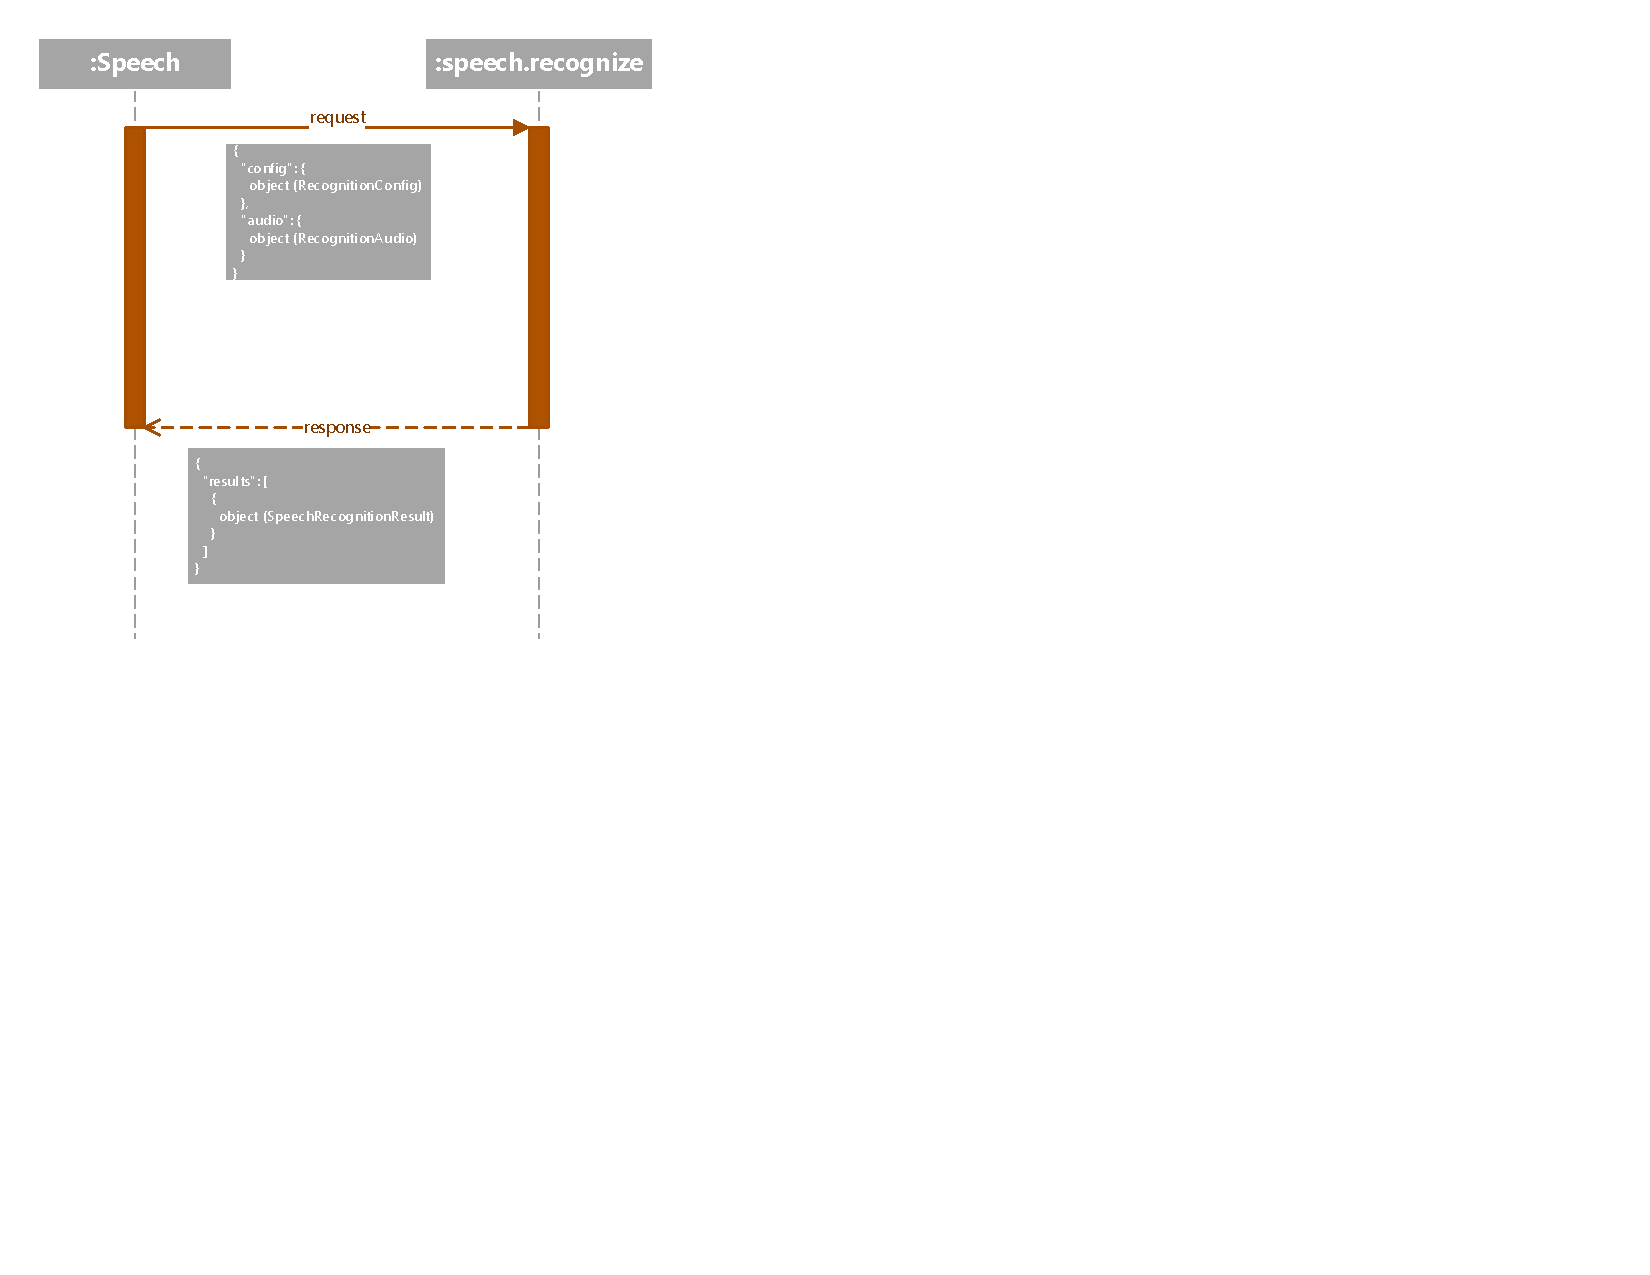
\includegraphics{uml/library_service_sequence_diagram.pdf}
\chapter{Βιβλιοθήκη Speech-to-Command}
\section{Σχεδίαση Βιβλιοθήκης}
\label{ch:σχεδίαση-βιβλιοθήκης}
\subsection{Διάγραμμα κλάσεων}\label{sec:διάγραμμα-κλάσεων}
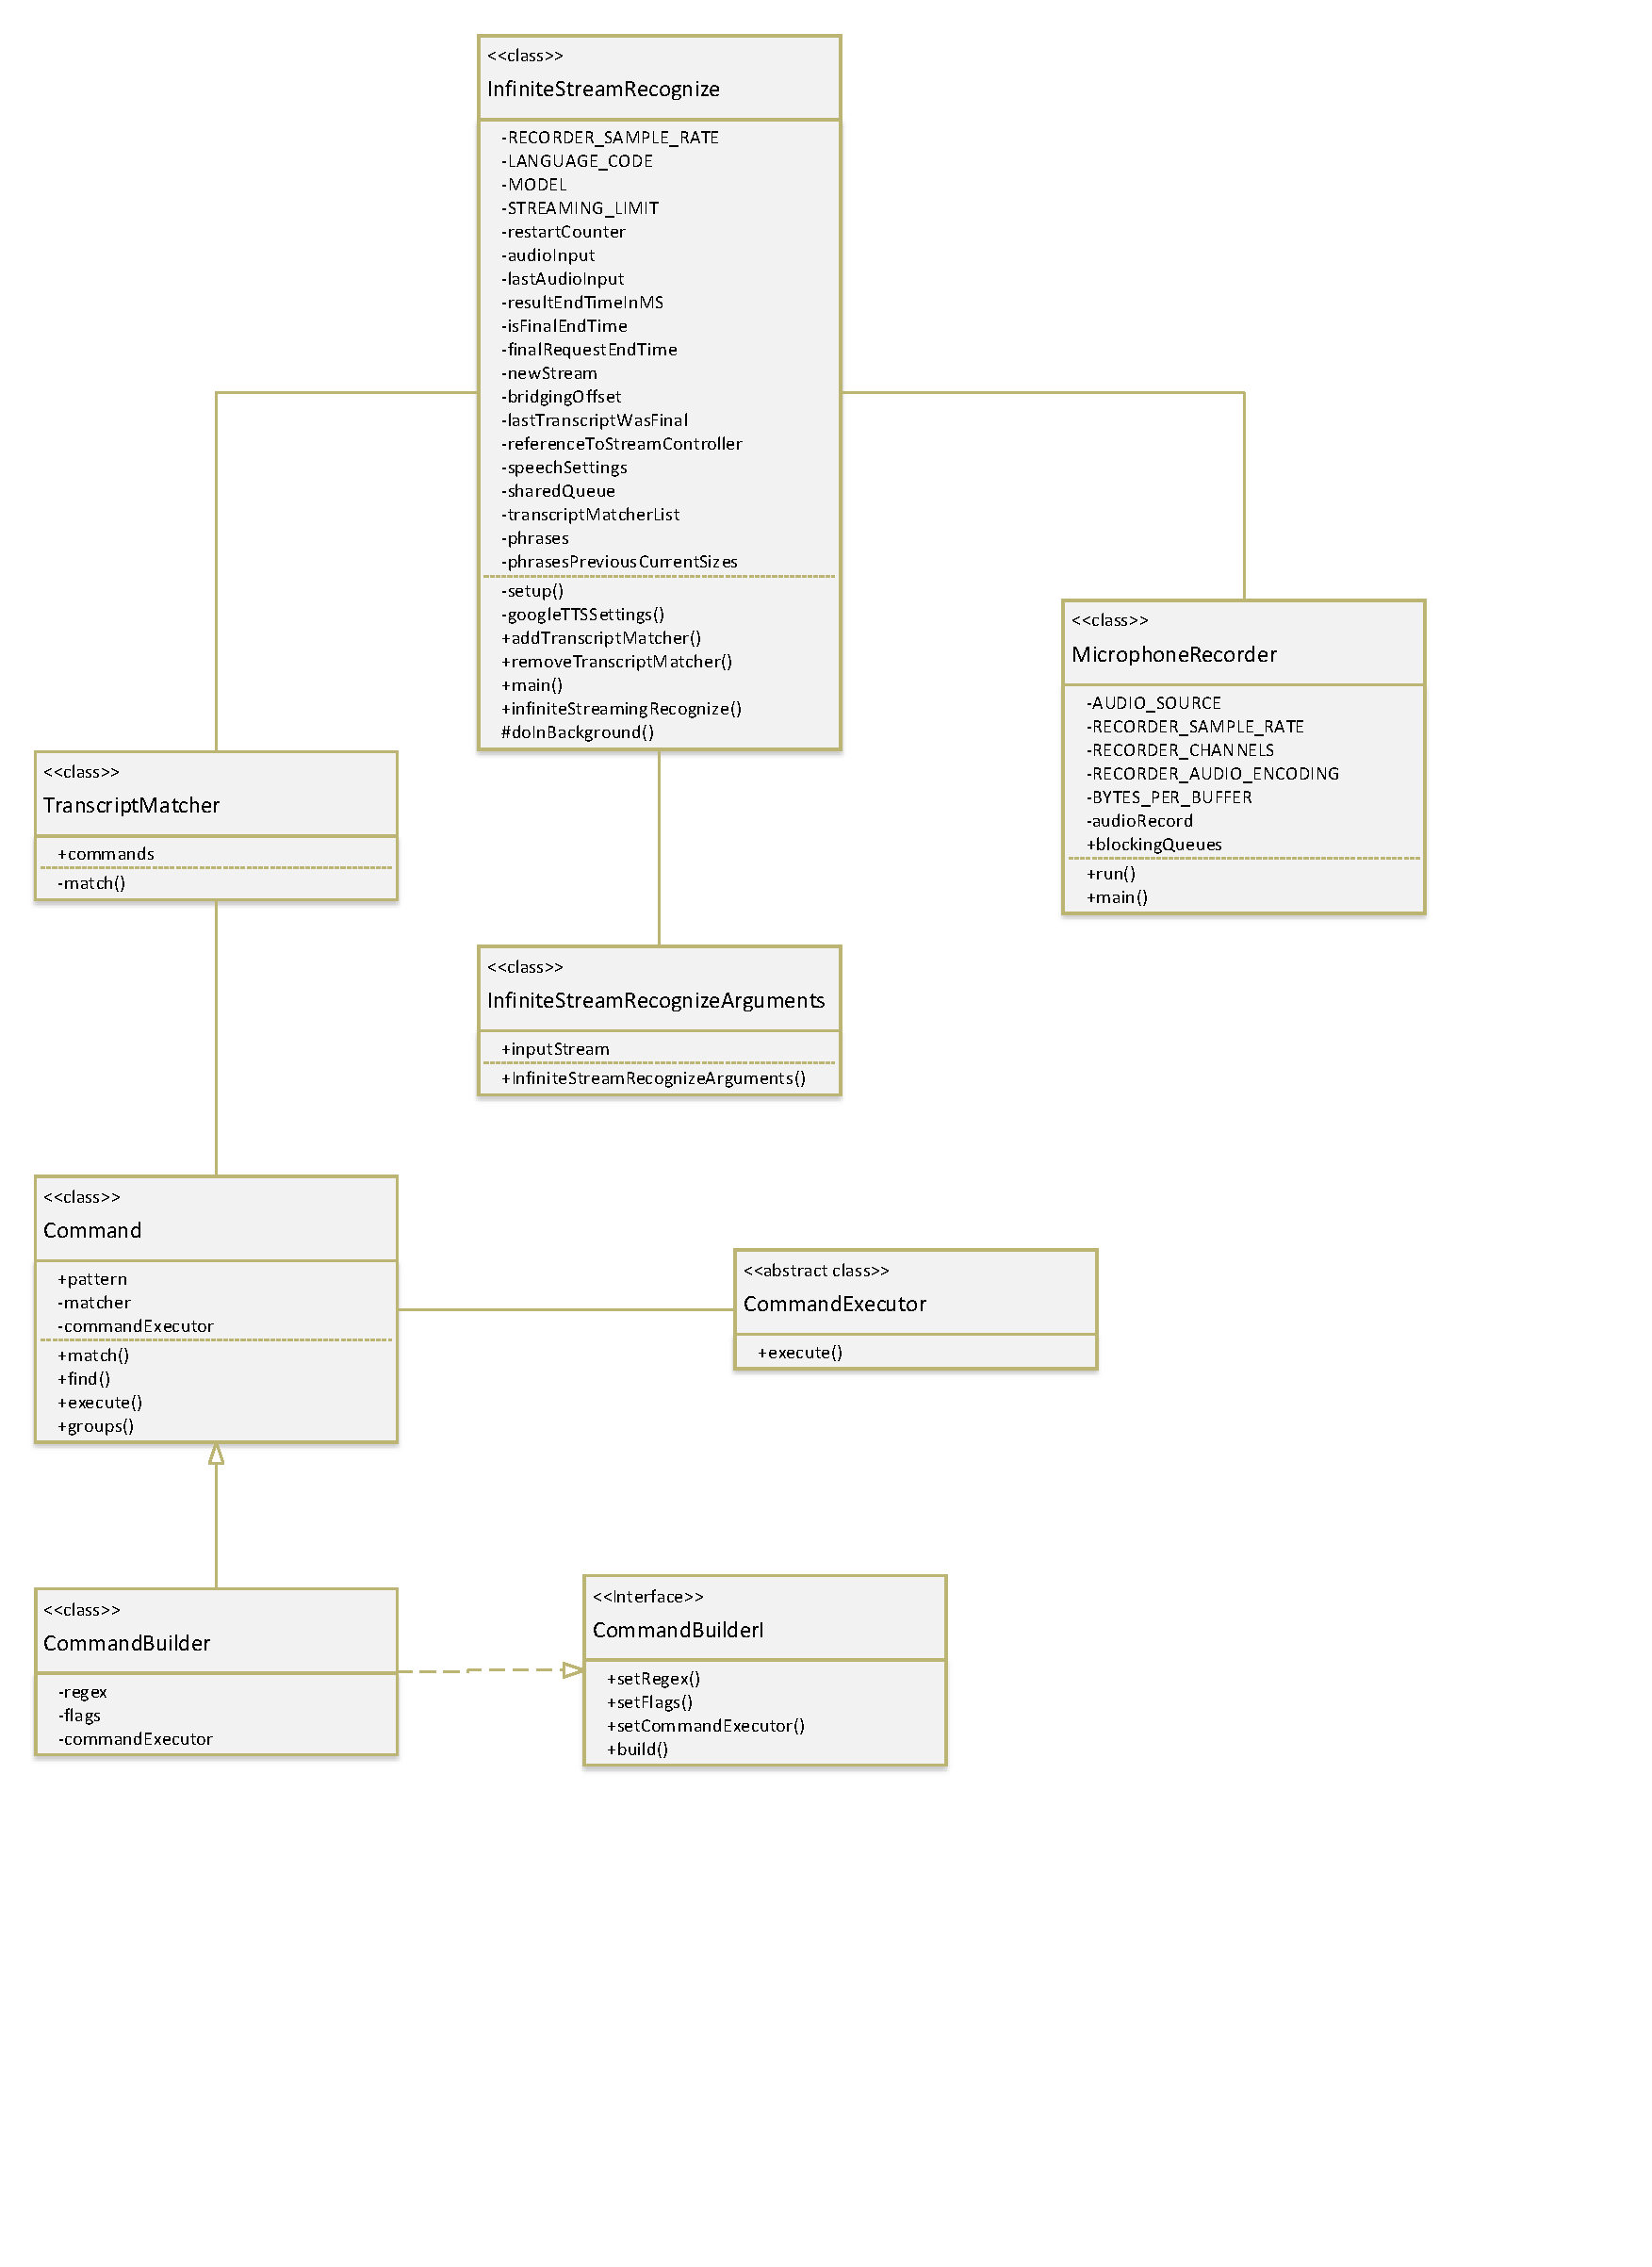
\includegraphics[scale=0.5]{uml/library_uml_class_diagram.pdf}
\subsection{Διάγραμμα σεναρίων χρήσης}\label{sec:διάγραμμα-σεναρίων-χρήσης}
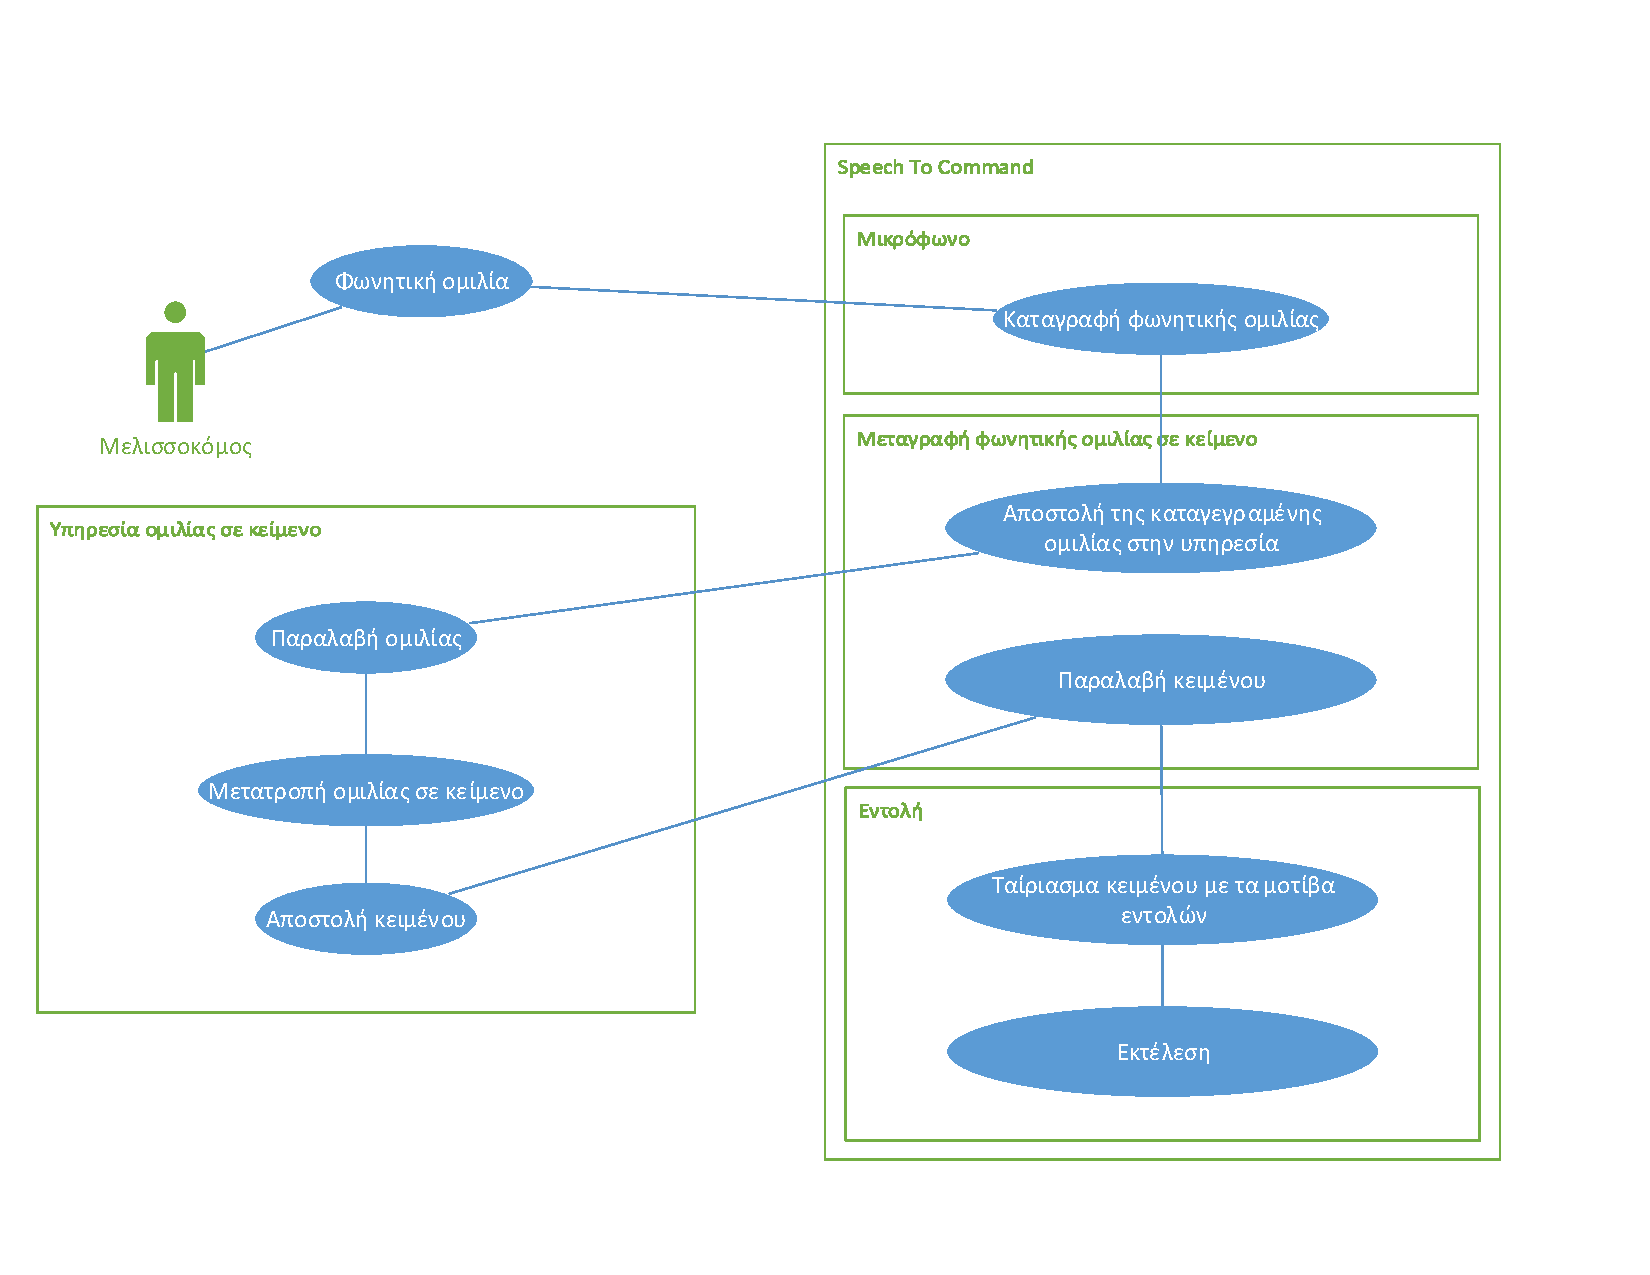
\includegraphics[scale=0.5]{uml/library_uml_use_case_diagram.pdf}
\subsection{Διάγραμμα συστατικών}\label{sec:διάγραμμα-συστατικών}
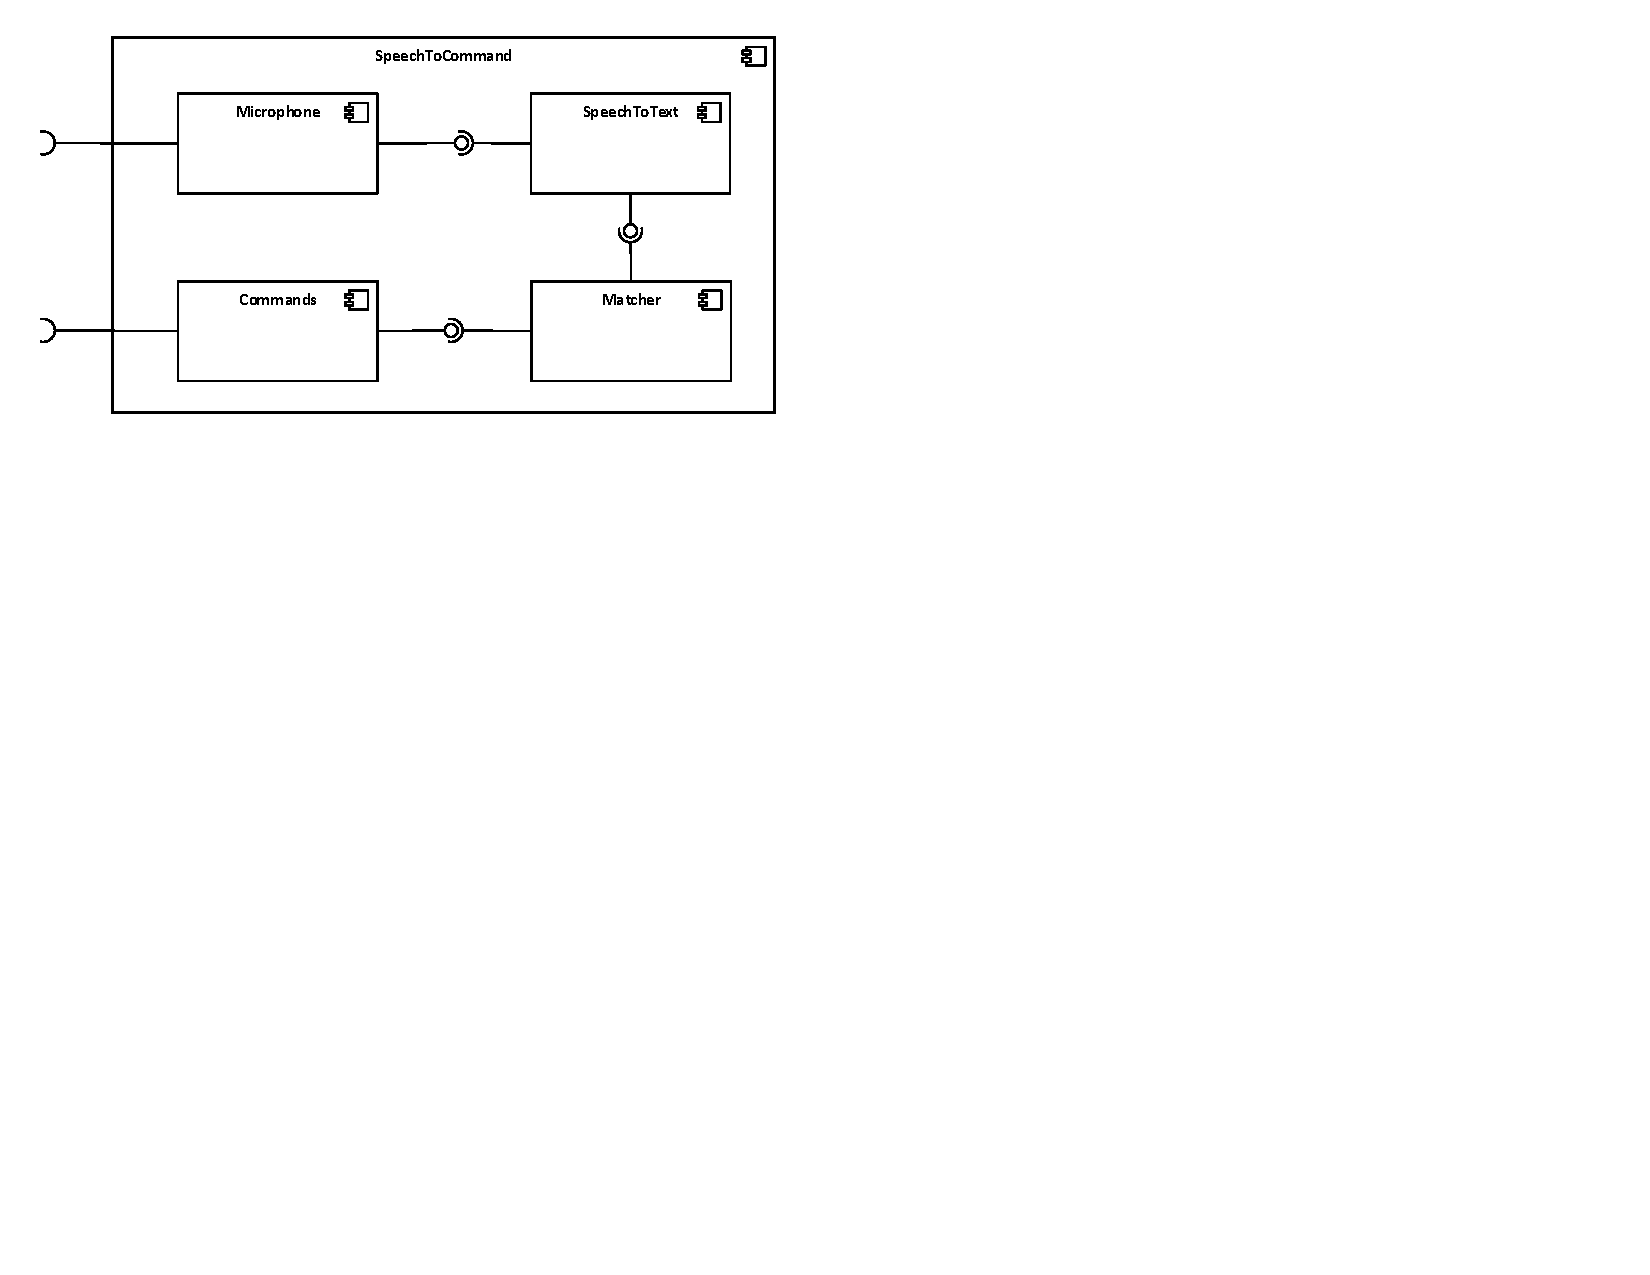
\includegraphics{uml/library_uml_component_diagram.pdf}
\section{Ανάπτυξη βιβλιοθήκης}
Η ανάπτυξη της βιβλιοθήκης έγινε στην γλώσσα προγραμματισμού Java για Android πλατφόρμα.Τα μέροι της βιβλιοθήκης είναι τα παρακάτω:
\begin{enumerate}
  \item Καταγραφή μικρόφωνου
  \item Speech-to-Text API αναγνώριση ροής
  \item Εντολή
  \item Εκτελεστής εντολών
  \item Ταιριαστής εντολών
\end{enumerate}
\subsection{Καταγραφή Μικροφώνου}
Η καταγραφή του μικροφώνου τρέχει σε ένα νήμα στην εφαρμογή, αποθηκεύοντας τα καταγεγραμμένα δεδομένα σε μία κοινόχρηστη ουρά.
\begin{center}
	Δείγμα κώδικα:
	\begin{lstlisting}[language=java]
public class MicrophoneRecorder extends Thread {
    private static final int AUDIO_SOURCE = MediaRecorder.AudioSource.UNPROCESSED;
    private static final int RECORDER_SAMPLE_RATE = 16000;
    private static final int RECORDER_CHANNELS = AudioFormat.CHANNEL_IN_MONO;
    private static final int RECORDER_AUDIO_ENCODING = AudioFormat.ENCODING_PCM_16BIT;
    private static final int BYTES_PER_BUFFER = 1600; // ~100ms
    private static AudioRecord audioRecord;
    public static volatile List<BlockingQueue<byte[]>> blockingQueues;

    @Override
    public void run() {
        audioRecord.startRecording();
        byte[] data = new byte[BYTES_PER_BUFFER];
        while (true) {
            try {
                int numBytesRead = audioRecord.read(data, 0, data.length);
                if ((numBytesRead <= 0)) {
                    continue;
                }
                for(BlockingQueue<byte[]> blockingQueue : blockingQueues){
                    blockingQueue.put(data.clone());
                }
            } catch (InterruptedException e) {
                System.out.println("Microphone input buffering interrupted : " + e.getMessage());
            }
        }
    }

    public static void main() {
        audioRecord = new AudioRecord(AUDIO_SOURCE,
                RECORDER_SAMPLE_RATE, RECORDER_CHANNELS,
                RECORDER_AUDIO_ENCODING, BYTES_PER_BUFFER);
        blockingQueues = new ArrayList<>();
        new MicrophoneRecorder().start();
    }
}
	\end{lstlisting}
\end{center}
\subsection{Speech-to-Text API αναγνώριση ροής}
Η αναγνώριση ροής τρέχει σε ένα ασύχρονο έργο στο παρασκήνιο, διαβάζοντας τα καταγεγραμμένα δεδομένα από την ουρά και κάνοντας συνέχες αιτήσεις στην υπηρεσία Speech-to-Text. Η υπηρεσία ανταποκρίνεται συνεχώς μέχρις ώτου έχει το τελικό αποτέλεσμα της μεταγραφής σε κείμενο της καταγεγραμμένης φωνητικής ομιλίας. Ο ταιριαστής των εντολών λαμβάνει την μεταγραφή ώστε να ταιριάξει το κείμενο.
\begin{center}
	Δείγμα κώδικα:
	\begin{lstlisting}[language=java]
public class InfiniteStreamRecognize extends AsyncTask<InfiniteStreamRecognizeArguments, Void, Void> {

    private static final int RECORDER_SAMPLE_RATE = 16000;
    private static final String LANGUAGE_CODE = "el-GR";
    private static final String MODEL = "command_and_search";

    private static final int STREAMING_LIMIT = 290000; // ~5 minutes

    public static final String RED = "\033[0;31m";
    public static final String GREEN = "\033[0;32m";
    public static final String YELLOW = "\033[0;33m";

    private static int restartCounter = 0;
    private static ArrayList<ByteString> audioInput = new ArrayList<>();
    private static ArrayList<ByteString> lastAudioInput = new ArrayList<>();
    private static int resultEndTimeInMS = 0;
    private static int isFinalEndTime = 0;
    private static int finalRequestEndTime = 0;
    private static boolean newStream = true;
    private static double bridgingOffset = 0;
    private static boolean lastTranscriptWasFinal = false;
    private static StreamController referenceToStreamController;
    private static SpeechSettings speechSettings;

    // Creating shared object
    private static volatile BlockingQueue<byte[]> sharedQueue = new LinkedBlockingQueue<>();
    private static volatile List<TranscriptMatcher> transcriptMatcherList = new ArrayList<>();
    private static List<String> phrases = new ArrayList<>();
    private static int[] phrasesPreviousCurrentSizes = {0, 0};


    private static void setup(InputStream is) throws IOException {
        MicrophoneRecorder.blockingQueues.add(sharedQueue);
        GoogleCredentials credentials = GoogleCredentials.fromStream(is);
        FixedCredentialsProvider credentialsProvider = FixedCredentialsProvider.create(credentials);

        speechSettings = SpeechSettings.newBuilder()
                .setCredentialsProvider(credentialsProvider)
                .build();
        googleSTTSettings();

    }

    private static StreamingRecognitionConfig googleSTTSettings(){
        phrasesPreviousCurrentSizes = new int[]{phrases.size(), phrases.size()};
        SpeechContext sc = SpeechContext.newBuilder().addAllPhrases(phrases).build();

        RecognitionMetadata rm = RecognitionMetadata.newBuilder()
                .setInteractionType(RecognitionMetadata.InteractionType.VOICE_COMMAND)
                .setMicrophoneDistance(RecognitionMetadata.MicrophoneDistance.NEARFIELD)
                .setOriginalMediaType(RecognitionMetadata.OriginalMediaType.AUDIO)
                .setRecordingDeviceType(RecognitionMetadata.RecordingDeviceType.SMARTPHONE)
                .build();

        RecognitionConfig recognitionConfig = RecognitionConfig.newBuilder()
                .setEncoding(RecognitionConfig.AudioEncoding.LINEAR16)
                .setSampleRateHertz(RECORDER_SAMPLE_RATE)
                .setLanguageCode(LANGUAGE_CODE)
                .setModel(MODEL)
                .addSpeechContexts(sc)
                .setMetadata(rm)
                .build();

        return StreamingRecognitionConfig.newBuilder()
                .setConfig(recognitionConfig)
                .setInterimResults(true)
//                .setSingleUtterance(true)
                .build();
    }

    public static void addTranscriptMatcher(TranscriptMatcher transcriptMatcher){
        transcriptMatcherList.add(transcriptMatcher);
        for(Command command: transcriptMatcher.commands){
            phrases.addAll(command.getPhrases());
        }
        phrasesPreviousCurrentSizes = new int[]{phrasesPreviousCurrentSizes[1], phrases.size()};
    }

    public static void removeTranscriptMatcher(TranscriptMatcher transcriptMatcher){
        transcriptMatcherList.remove(transcriptMatcher);
        for(Command command: transcriptMatcher.commands){
            phrases.removeAll(command.getPhrases());
        }
        phrasesPreviousCurrentSizes = new int[]{phrasesPreviousCurrentSizes[1], phrases.size()};
    }

    public static void main(InputStream is) {
        try {
            setup(is);
            infiniteStreamingRecognize();
        } catch (Exception e) {
            System.out.println("Exception caught: " + e);
        }
    }

    public static String convertMillisToDate(double milliSeconds) {
        long millis = (long) milliSeconds;
        DecimalFormat format = new DecimalFormat();
        format.setMinimumIntegerDigits(2);
        return String.format(
                "%s:%s /",
                format.format(TimeUnit.MILLISECONDS.toMinutes(millis)),
                format.format(
                        TimeUnit.MILLISECONDS.toSeconds(millis)
                                - TimeUnit.MINUTES.toSeconds(TimeUnit.MILLISECONDS.toMinutes(millis))));
    }

    /** Performs infinite streaming speech recognition */
    public static void infiniteStreamingRecognize() throws Exception {
        ResponseObserver<StreamingRecognizeResponse> responseObserver;

        try (SpeechClient client = SpeechClient.create(speechSettings)) {
            ClientStream<StreamingRecognizeRequest> clientStream;
            responseObserver = new ResponseObserver<StreamingRecognizeResponse>() {
                ArrayList<StreamingRecognizeResponse> responses = new ArrayList<>();

                public void onStart(StreamController controller) {
                    referenceToStreamController = controller;
                }

                public void onResponse(StreamingRecognizeResponse response) {
                    responses.add(response);
                    StreamingRecognitionResult result = response.getResultsList().get(0);
                    Duration resultEndTime = result.getResultEndTime();
                    resultEndTimeInMS =
                            (int)
                                    ((resultEndTime.getSeconds() * 1000) + (resultEndTime.getNanos() / 1000000));
                    double correctedTime =
                            resultEndTimeInMS - bridgingOffset + (STREAMING_LIMIT * restartCounter);

                    SpeechRecognitionAlternative alternative = result.getAlternativesList().get(0);
                    if (result.getIsFinal()) {
                        for(TranscriptMatcher transcriptMatcher : transcriptMatcherList){
                            transcriptMatcher.match(alternative.getTranscript().trim());
                        }
                        System.out.print(GREEN);
                        System.out.print("\033[2K\r");
                        System.out.printf(
                                "%s: %s [confidence: %.2f]\n",
                                convertMillisToDate(correctedTime),
                                alternative.getTranscript(),
                                alternative.getConfidence());
                        isFinalEndTime = resultEndTimeInMS;
                        lastTranscriptWasFinal = true;
                    } else {
                        System.out.print(RED);
                        System.out.print("\033[2K\r");
                        System.out.printf(
                                "%s: %s", convertMillisToDate(correctedTime), alternative.getTranscript());
                        lastTranscriptWasFinal = false;
                    }
                }

                public void onComplete() {
                    System.out.println("COMPLETEEEEEE");
                }

                public void onError(Throwable t) {
                    System.out.println(t.getMessage());
                }
            };
            clientStream = client.streamingRecognizeCallable().splitCall(responseObserver);

            StreamingRecognitionConfig streamingRecognitionConfig = googleSTTSettings();
            StreamingRecognizeRequest request =
                    StreamingRecognizeRequest.newBuilder()
                            .setStreamingConfig(streamingRecognitionConfig)
                            .build(); // The first request in a streaming call has to be a config

            clientStream.send(request);

            try {
                long startTime = System.currentTimeMillis();

                while (true) {

                    long estimatedTime = System.currentTimeMillis() - startTime;

                    if (estimatedTime >= STREAMING_LIMIT || (phrasesPreviousCurrentSizes[0] != phrasesPreviousCurrentSizes[1])) {

                        clientStream.closeSend();
                        referenceToStreamController.cancel(); // remove Observer

                        if (resultEndTimeInMS > 0) {
                            finalRequestEndTime = isFinalEndTime;
                        }
                        resultEndTimeInMS = 0;

                        lastAudioInput = null;
                        lastAudioInput = audioInput;
                        audioInput = new ArrayList<>();

                        restartCounter++;

                        if (!lastTranscriptWasFinal) {
                            System.out.print('\n');
                        }

                        newStream = phrasesPreviousCurrentSizes[0] == phrasesPreviousCurrentSizes[1];

                        clientStream = client.streamingRecognizeCallable().splitCall(responseObserver);
                        streamingRecognitionConfig = googleSTTSettings();
                        request =
                                StreamingRecognizeRequest.newBuilder()
                                        .setStreamingConfig(streamingRecognitionConfig)
                                        .build();

                        System.out.println(YELLOW);
                        System.out.printf("%d: RESTARTING REQUEST\n", restartCounter * STREAMING_LIMIT);

                        startTime = System.currentTimeMillis();

                    } else {

                        if ((newStream) && (lastAudioInput.size() > 0)) {
                            // if this is the first audio from a new request
                            // calculate amount of unfinalized audio from last request
                            // resend the audio to the speech client before incoming audio
                            double chunkTime = STREAMING_LIMIT / lastAudioInput.size();
                            // ms length of each chunk in previous request audio arrayList
                            if (chunkTime != 0) {
                                if (bridgingOffset < 0) {
                                    // bridging Offset accounts for time of resent audio
                                    // calculated from last request
                                    bridgingOffset = 0;
                                }
                                if (bridgingOffset > finalRequestEndTime) {
                                    bridgingOffset = finalRequestEndTime;
                                }
                                int chunksFromMS =
                                        (int) Math.floor((finalRequestEndTime - bridgingOffset) / chunkTime);
                                // chunks from MS is number of chunks to resend
                                bridgingOffset =
                                        (int) Math.floor((lastAudioInput.size() - chunksFromMS) * chunkTime);
                                // set bridging offset for next request
                                for (int i = chunksFromMS; i < lastAudioInput.size(); i++) {
                                    request =
                                            StreamingRecognizeRequest.newBuilder()
                                                    .setAudioContent(lastAudioInput.get(i))
                                                    .build();
                                    clientStream.send(request);
                                }
                            }
                            newStream = false;
                        }

                        ByteString tempByteString = ByteString.copyFrom(sharedQueue.take());

                        request =
                                StreamingRecognizeRequest.newBuilder().setAudioContent(tempByteString).build();

                        audioInput.add(tempByteString);
                    }

                    clientStream.send(request);
                }
            } catch (Exception e) {
                System.out.println(e.getMessage());
            }
        }
    }

    @Override
    protected Void doInBackground(InfiniteStreamRecognizeArguments... infiniteStreamRecognizeArguments) {
        try {
            setup(infiniteStreamRecognizeArguments[0].inputStream);
            infiniteStreamingRecognize();
        } catch (Exception e) {
            System.out.println("Exception caught: " + e);
        }
        return null;
    }
}
	\end{lstlisting}
\end{center}
\subsection{Εντολή}
Η εντολή αποτελείται από μία κανονική έκφραση η οποία είναι μια ακολουθία χαρακτήρων που ορίζουν ένα μοτίβο αναζήτησης, από τον κώδικα που θα εκτελεστεί αν το μοτίβο ταιριάξει με την μεταγραφή απο το Speech-to-Text API και μια λίστα λέξεων και φράσεων που παρέχουν συμβουλές στην υπηρεσία για την εργασία αναγνώρισης ομιλίας.
\begin{center}
	Δείγμα κώδικα:
	\begin{lstlisting}[language=java]
public class Command {
    public Pattern pattern;
    private Matcher matcher;
    private CommandExecutor commandExecutor;
    private List<String> phrases;

    public Command(String regex, CommandExecutor commandExecutor, int flags, List<String> phrases){
        this.commandExecutor = commandExecutor;
        this.phrases = phrases;
        try{
            pattern = Pattern.compile(regex, flags);
        }
        catch(PatternSyntaxException pSE){
            System.out.println("Incorrect Regular Expression: " + pSE.getMessage());
        }
    }

    public Boolean match(String text){
        matcher = pattern.matcher(text);
        return matcher.matches();
    }

    public Boolean find(String text){
        matcher = pattern.matcher(text);
        return matcher.find();
    }

    public void execute(List<String> list){
        commandExecutor.execute(list);
    }

    public List<String> groups(){
        List<String> groups = new ArrayList<>();
        if(matcher != null){
            int noGroups = matcher.groupCount();
            for(int i=0; i <= noGroups; i++) {
                groups.add(matcher.group(i));
            }
        }
        else{
            System.out.println("Couldn't match!");
        }
        return groups;
    }

    public List<String> getPhrases(){
        if(phrases == null){
            phrases = new ArrayList<>();
        }
        return phrases;
    }
}
	\end{lstlisting}
\end{center}
\subsection{Εκτελεστής Εντολών}
Ο εκτελεστής εντολών εκτελεί τη συνάρτηση που δηλώνεται όταν το μοτίβο της εντολής ταιριάξει με την μεταγραφή απο την υπηρεσία Speech-to-Text.
\begin{center}
	Δείγμα κώδικα:
	\begin{lstlisting}[language=java]
public abstract class CommandExecutor {

     public abstract void execute(List<String> list);
}
	\end{lstlisting}
\end{center}
\subsection{Ταιριαστής Εντολών}
Ο ταιριαστής εντολών ταιριάζει την μεταγραφή απο την υπηρεσία Speech-to-Text πάνω στο μοτίβο και καλεί τον εκτελεστή εντολών αν ταιριάξει επιτυχώς.
\begin{center}
	Δείγμα κώδικα:
	\begin{lstlisting}[language=java]
public class TranscriptMatcher {
    public List<Command> commands;

    public TranscriptMatcher(List<Command> commands){
        this.commands = commands;
    }

    public void match(String transcript){
        for(Command command : commands){
            if(command.match(transcript)){
                command.execute(command.groups());
                break;
            }
        }
    }
}
	\end{lstlisting}
\end{center}
\chapter{Μελισσοκομική Εφαρμογή}
Η εφαρμογή είναι το πρακτικό παράδειγμα χρήσης της βιβλιοθήκης Speech-to-Command.
\section{Υλοποιήση φωνητικών εντολών}
Δείγμα κώδικα της υλοποιήσης των φωνητικών εντολών:
\begin{itemize}
	\item Μελίσσι
	\begin{lstlisting}[language=java]
Command melissiCommand = new CommandBuilder().setCommandExecutor(new CommandExecutor() {
            @Override
            public void execute(List<String> list) {
                Beehive beehive = db.beehiveDao().findBeehiveId(Integer.parseInt(list.get(1)));
                if(beehive != null) {
                    Intent intent = new Intent(MainActivity.this, BeehiveChecksActivity.class);
                    intent.putExtra(BeehiveChecksActivity.EXTRA_BEEHIVE_NUMBER, beehive.number);
                    intent.putExtra(BeehiveChecksActivity.EXTRA_BEEHIVE_ID, beehive.id);
                    MainActivity.this.startActivity(intent);
                }
                else {
                    Toast.makeText(MainActivity.this, "Μελίσσι "+list.get(1)+" δεν υπάρχει!", Toast.LENGTH_LONG).show();
                }
            }
        }).setRegex("μελ[ιί]σσι\\s+(\\d+)").setFlags(Pattern.CASE_INSENSITIVE|Pattern.DOTALL)
                .setPhrases(beehivePhrases).build();
	\end{lstlisting}
    \item Πλαίσια
	\begin{lstlisting}[language=java]
	Command frameCommand = new CommandBuilder().setCommandExecutor(new CommandExecutor() {
            @Override
            public void execute(final List<String> list) {
                Log.i("Πλαισια:", list.get(1));
                NewEditBeehiveCheckActivity.this.runOnUiThread(new Runnable() {
                    public void run() {
                        editFrames.setText(list.get(1));
                        Toast.makeText(NewEditBeehiveCheckActivity.this, "Πλαίσιο " + list.get(1) + "!", Toast.LENGTH_LONG).show();
                    }
                });
            }
        }).setRegex("πλα[ιί]σι[οα]\\s+(\\d+)").setFlags(Pattern.CASE_INSENSITIVE | Pattern.DOTALL)
                .setPhrases(framePhrases).build();
    \end{lstlisting}
    \item Πλυθησμός
	\begin{lstlisting}[language=java]
	Command populationCommand = new CommandBuilder().setCommandExecutor(new CommandExecutor() {
            @Override
            public void execute(final List<String> list) {
                Log.i("Πληθυσμός:", list.get(1));
                NewEditBeehiveCheckActivity.this.runOnUiThread(new Runnable() {
                    public void run() {
                        editPopulation.setText(list.get(1));
                        Toast.makeText(NewEditBeehiveCheckActivity.this, "Πληθυσμός " + list.get(1) + "!", Toast.LENGTH_LONG).show();
                    }
                });
            }
        }).setRegex("πληθυσμ[οό]ς\\s+(\\d+)").setFlags(Pattern.CASE_INSENSITIVE | Pattern.DOTALL)
                .setPhrases(populationPhrases).build();
	\end{lstlisting}
	\item Γόνος
	\begin{lstlisting}[language=java]
	Command progenyCommand = new CommandBuilder().setCommandExecutor(new CommandExecutor() {
            @Override
            public void execute(final List<String> list) {
                Log.i("ΓΟΝΟΣ:", list.get(1));
                NewEditBeehiveCheckActivity.this.runOnUiThread(new Runnable() {
                    public void run() {
                        editProgeny.setText(list.get(1));
                        Toast.makeText(NewEditBeehiveCheckActivity.this, "ΓΟΝΟΣ " + list.get(1) + "!", Toast.LENGTH_LONG).show();
                    }
                });
            }
        }).setRegex("γ[όο]νος\\s+(\\d+)").setFlags(Pattern.CASE_INSENSITIVE | Pattern.DOTALL)
                .setPhrases(progenyPhrases).build();
	\end{lstlisting}
	\item Μέλι
	\begin{lstlisting}[language=java]
	Command honeyCommand = new CommandBuilder().setCommandExecutor(new CommandExecutor() {
            @Override
            public void execute(final List<String> list) {
                Log.i("Μέλι:", list.get(1));
                NewEditBeehiveCheckActivity.this.runOnUiThread(new Runnable() {
                    public void run() {
                        editHoney.setText(list.get(1));
                        Toast.makeText(NewEditBeehiveCheckActivity.this, "Μέλι " + list.get(1) + "!", Toast.LENGTH_LONG).show();
                    }
                });
            }
        }).setRegex("μ[έε]λι\\s+(\\d+)").setFlags(Pattern.CASE_INSENSITIVE | Pattern.DOTALL)
                .setPhrases(honeyPhrases).build();
	\end{lstlisting}
	\item Γύρη
	\begin{lstlisting}[language=java]
	 Command pollenCommand = new CommandBuilder().setCommandExecutor(new CommandExecutor() {
            @Override
            public void execute(final List<String> list) {
                Log.i("Γύρη:", list.get(1));
                NewEditBeehiveCheckActivity.this.runOnUiThread(new Runnable() {
                    public void run() {
                        editPollen.setText(list.get(1));
                        Toast.makeText(NewEditBeehiveCheckActivity.this, "Γύρη " + list.get(1) + "!", Toast.LENGTH_LONG).show();
                    }
                });
            }
        }).setRegex("γ[ύυ]ρη\\s+(\\d+)").setFlags(Pattern.CASE_INSENSITIVE | Pattern.DOTALL)
                .setPhrases(pollenPhrases).build();
	\end{lstlisting}
	\item Παρατήρηση
	\begin{lstlisting}[language=java]
	 Command noteCommand = new CommandBuilder().setCommandExecutor(new CommandExecutor() {
            @Override
            public void execute(final List<String> list) {
                Log.i("Παρατήρηση:", list.get(1));
                NewEditBeehiveCheckActivity.this.runOnUiThread(new Runnable() {
                    public void run() {
                        if(editNotes.getText().length() > 0){
                            editNotes.append("," + list.get(1));
                        }
                        else{
                            editNotes.setText(list.get(1));
                        }
                        Toast.makeText(NewEditBeehiveCheckActivity.this, "Παρατήρηση " + list.get(1) + "!", Toast.LENGTH_LONG).show();
                    }
                });
            }
        }).setRegex("παρατ[ήη]ρηση\\s+(.*)").setFlags(Pattern.CASE_INSENSITIVE | Pattern.DOTALL)
                .setPhrases(notesPhrases).build();
	\end{lstlisting}
\end{itemize}
\section{Παράδειγμα χρήσης}
Τo παρακάτω παράδειγμα χρήσης είναι για την δοκιμή των υπηρεσιών της βιβλιοθήκης μέσω της εφαρμογής. Σε αυτό το παράδειγμα υλοποιείται μια φυσιολογική ροή με σωστή χρήση των φωνητικών εντολών.
Κεντρικό γραφικό
\begin{figure}[H]
    \centering
    \includegraphics[scale=0.3]{images/app_screenshot_1.jpg}
    \caption{Κεντρικό γραφικό της εφαρμογής}
    \label{fig:myfigure}
\end{figure}
Έναρξη νέου ελέγχου μελισσιού μέσω φωνητικών εντολών:
\newline
Φωνητική εντολή: Μελίσσι 1
\newline
Γραφικό:
\begin{figure}[H]
    \centering
    \includegraphics[scale=0.3]{images/app_screenshot_2.jpg}
    \caption{Νέος έλεγχος μελισσιού}
    \label{fig:myfigure}
\end{figure}
\newpage
Φωνητικές εντολές για το γέμιστα των πεδιών του γραφικού
\begin{enumerate}
	\item Φωνητική εντολή: Πλαίσια 10
	\begin{figure}[H]
    	\centering
    	\includegraphics[scale=0.3]{images/app_screenshot_3.jpg}
    	\caption{Προσθήκη αριθμού πλαισίων}
	\end{figure}
	\newpage
	\item Φωνητική εντολή: Πλυθησμός 8
	\begin{figure}[H]
    	\centering
    	\includegraphics[scale=0.3]{images/app_screenshot_4.jpg}
    	\caption{Προσθήκη αριθμού πλαισίων πλυθησμού}
	\end{figure}
	\newpage
	\item Φωνητική εντολή: Γόνος 3
	\begin{figure}[H]
    	\centering
    	\includegraphics[scale=0.3]{images/app_screenshot_5.jpg}
    	\caption{Προσθήκη αριθμού πλαισίων γόνου}
	\end{figure}
	\newpage
	\item Φωνητική εντολή: Μέλι 2
	\begin{figure}[H]
    	\centering
    	\includegraphics[scale=0.3]{images/app_screenshot_6.jpg}
    	\caption{Προσθήκη αριθμού πλαισίων μελιού}
	\end{figure}
	\newpage
	\item Φωνητική εντολή: Γύρη 3
	\begin{figure}[H]
    	\centering
    	\includegraphics[scale=0.3]{images/app_screenshot_7.jpg}
    	\caption{Προσθήκη αριθμού πλαισίων γύρης}
	\end{figure}
	\newpage
	\item Φωνητική εντολή: Παρατήρηση θέλει νέο όροφο
	\begin{figure}[H]
    	\centering
    	\includegraphics[scale=0.3]{images/app_screenshot_8.jpg}
    	\caption{Προσθήκη παρατήρησης}
	\end{figure}
\end{enumerate}
\chapter{Συμπεράσματα}
\section{Στόχοι}
Κατά την διάρκεια εκπόνησης της πτυχιακής εργασίας, επιτεύχθηκε ο κύριος στόχος που αρχικά είχαμε θέσει, αυτός της δημιουργίας μιας βιβλιοθήκης και μιας εφαρμογή που την χρησιμοποιεί. Η δημιουργία της βιβλιοθήκης και της εφαρμογής δεν ήταν οι μοναδικοί στόχοι που επιτεύχθηκαν. Σε προσωπικό επίπεδο τα κέρδη ήταν πολλαπλά. Η μελέτη και η έρευνα της βιβλιογραφίας σε τέτοιο βαθμό ήταν κάτι πρωτόγνωρο αλλά και παράλληλα εποικοδομητική καθώς βάσει αυτής γράφτηκε το παρόν βιβλίο με τις όποιες τεκμηριώσεις. Επίσης η αναπτύξη αυτού του εργαλειού μπορεί να εφαρμοστεί σε πραγματικά προβλήματα όπως αυτά του μελισσοκόμου που σύμβαλε στην ανάπτυξη της εφαρμαγής για την δοκιμή της βιβλιοθήκης.
\section{Δυσκολίες}
Κατά την διάρκεια ανάπτυξης της εργασίας, η μοναδικη δυσκολία που παρουσιάστηκε ήταν τεχνικής φύσεως. Συγκεκριμένα, στην ανάπτυξη της βιβλιοθήκης έτσι ώστε να είναι φιλική προς τον προγραμματιστή όταν την χρησιμοποιήσει.
\section{Προτάσεις εξέλιξεις}
Όπως είναι φυσιολογικό, η βιβλιοθήκη επιδέχεται βελτίωσης αλλά και νέων προσθηκών που θα το κάνουν πιο δυναμικό αλλά και πιο φιλικό προς τον χρήστη. Ο πηγαίος κώδικας όπως και οποιαδήποτε πρόσθετη πληροφορία υπάρχει στην διεύθυνση \path{https://github.com/EvanPetr/Thesis}
Αναφορικά μερικές προτάσεις εξέλιξης είναι οι εξής:
\begin{itemize}
	\item Δημιουργία κλάσεων για τα exceptions της βιβλιοθήκης για την καλύτερη καθοδήγηση του χρήστη στην επίλυση των προβλημάτων.
	\item Δυνατότητα χρησιμοποιήσεις διαφορετικού Speech-to-text API από αυτό της Google.
	\item Υλοποιήση Testing στην βιβλιοθήκη για πρόληψη σφάλματων.
\end{itemize}


\begin{Glossary}
\begin{description}
  \item[AI]Artificial Intelligence
  \item[API]Application Programming Interface
  \item[GUI]Graphical User Interface
  \item[REST]REpresentational State Transfer
  \item[gRPC]google Remote Procedure Calls
  \item[FLAC]Free Lossless Audio Codec
  \item[WAV]Waveform Audio File Format
  \item[URI]Uniform Resource Identifier
  \item[ASR]Automatic Speech Recognition
\end{description}
\end{Glossary}
\newpage
\nocite{*}
\printbibliography
\lastpageinfo
\end{document}
